% ============================================================================
%  KMUTT GRADUATE THESIS PROPOSAL  (ENGLISH)
%  Cross-Embodiment Locomotion Transfer from Egocentric Visual World Model without Prior Knowledge of the Morphology
%  Content migrated from report/report_proposal.md (2026).
%  Compile with pdfLaTeX (run twice for Contents / cross-refs).
%  NOTE: the Thai abstract renders only under XeLaTeX/LuaLaTeX (a Thai font is
%  loaded conditionally below); under pdfLaTeX it prints a one-line placeholder.
% ============================================================================
\documentclass[12pt,a4paper,oneside]{report}

\usepackage{iftex}

% ---- Thai support (XeLaTeX / LuaLaTeX only) --------------------------------
% fontspec MUST load before newtx: newtx-before-fontspec breaks fontspec's
% font-by-name lookup under XeLaTeX. Compile with XeLaTeX to render the Thai
% abstract (Overleaf: Menu -> Compiler -> XeLaTeX).
\newif\ifThai\Thaifalse
\ifXeTeX\Thaitrue\fi
\ifLuaTeX\Thaitrue\fi
\ifThai
  \usepackage{fontspec}
  % Thai abstract uses TH Sarabun New (the KMUTT / Thai-official standard). It runs
  % small next to newtx, so match its x-height to the Latin text. Fall back to
  % Noto Sans Thai, then Norasi (TLWG), if TH Sarabun New is not installed.
  \IfFontExistsTF{TH Sarabun New}
    {\newfontfamily\thaifont{TH Sarabun New}[Scale=MatchLowercase]}
    {\IfFontExistsTF{Noto Sans Thai}
      {\newfontfamily\thaifont{Noto Sans Thai}[Scale=MatchLowercase]}
      {\newfontfamily\thaifont{Norasi}[Scale=MatchLowercase]}}
\fi

\ifpdftex
  \usepackage[T1]{fontenc}     % pdfLaTeX only (not needed / harmful under XeLaTeX-LuaLaTeX)
  \usepackage[utf8]{inputenc}
\fi
\usepackage{amsmath}
\usepackage{newtxtext,newtxmath}   % Times New Roman-compatible text + math (all engines)
% newtx's own typewriter shape (t1xtt, from txfonts) is not installed in this TeX distribution,
% which makes any \texttt fatal under pdfLaTeX. Latin Modern's typewriter shape is a standard
% part of every TeX install (no extra package, so no further missing-dependency risk) and is
% used for \ttfamily instead of falling back to the mismatched Computer Modern typewriter.
\renewcommand{\ttdefault}{lmtt}

% ---- Page geometry: exact KMUTT margins [p.41] ------------------------------
\usepackage[a4paper,top=30mm,left=40mm,right=20mm,bottom=20mm]{geometry}

% ---- Line spacing: single --------------------------------------------------
\usepackage{setspace}
\singlespacing

\usepackage{graphicx}
\usepackage{caption}
\usepackage{float}
\usepackage{array}
\newcolumntype{P}[1]{>{\raggedright\arraybackslash\hyphenpenalty=10000\exhyphenpenalty=10000}p{#1}}
\usepackage{tabularx}
% Y: a stretchy version of P, used with tabularx so every multi-column table fills the full text
% width automatically instead of being sized by hand-summed column widths (which is where every
% earlier "too narrow" / overfull-hbox mistake in this document came from). Per-column relative
% width is set with the standard tabularx idiom >{\hsize=<n>\hsize}Y, chosen so the factors in one
% row sum to the column count.
\newcolumntype{Y}{>{\raggedright\arraybackslash\hyphenpenalty=10000\exhyphenpenalty=10000}X}
\usepackage{indentfirst}
\usepackage{enumitem}
\setlist{topsep=0pt, itemsep=0pt, parsep=0pt, partopsep=0pt}
\setlength{\parskip}{6pt plus 2pt minus 1pt}
\setlength{\parindent}{2.5em}
\makeatletter
\g@addto@macro\normalsize{%
  \setlength\baselineskip{17pt}%
  \setlength\abovedisplayskip{7pt plus 2pt minus 1pt}%
  \setlength\belowdisplayskip{3pt plus 2pt minus 1pt}%
  \setlength\abovedisplayshortskip{5pt plus 2pt minus 1pt}%
  \setlength\belowdisplayshortskip{2pt plus 1pt minus 1pt}%
}
\makeatother
\hyphenpenalty=100
\exhyphenpenalty=100
\tolerance=100
\emergencystretch=3em
\usepackage{titlesec}
\usepackage{fancyhdr}
\usepackage[hidelinks]{hyperref}
\makeatletter
\renewcommand{\@dotsep}{10000}
\makeatother

% ---- Heading sizes: chapter 15 / section 14 / subsection 13, all bold [p.41]-
\titleformat{\chapter}[block]
  {\filcenter\bfseries\fontsize{15}{18}\selectfont}
  {\MakeUppercase{\chaptername}\ \thechapter}{1ex}{}
\titlespacing*{\chapter}{0pt}{0pt}{14pt}

\titleformat{\section}
  {\bfseries\fontsize{14}{18}\selectfont}{\thesection}{1ex}{}
\titlespacing*{\section}{0pt}{12pt plus 2pt minus 2pt}{4pt}

\titleformat{\subsection}
  {\bfseries\fontsize{13}{18}\selectfont}{\thesubsection}{1ex}{}
\titlespacing*{\subsection}{0pt}{9pt plus 2pt minus 2pt}{3pt}

% ---- Page numbering: top-right; none on a chapter's first page [p.12] --------
\pagestyle{fancy}
\fancyhf{}
\fancyhead[R]{\thepage}
\renewcommand{\headrulewidth}{0pt}
\fancypagestyle{plain}{\fancyhf{}\renewcommand{\headrulewidth}{0pt}}

\captionsetup{labelfont=bf, labelsep=space, aboveskip=10pt, belowskip=-7pt}
\captionsetup[table]{singlelinecheck=false}
\setlength{\intextsep}{10pt plus 2pt minus 2pt}
\setlength{\textfloatsep}{12pt plus 2pt minus 2pt}

\renewcommand{\bibname}{References}

% ---- ToC: a little breathing space before each section (x.x) line -----------
\makeatletter
\let\oldl@section\l@section
\renewcommand{\l@section}[2]{\addvspace{5pt}\oldl@section{#1}{#2}}
\makeatother

% ---- List of Tables / Figures: all-caps title + TABLE/FIGURE ... PAGE header
\renewcommand{\listtablename}{LIST OF TABLES}
\renewcommand{\listfigurename}{LIST OF FIGURES}
\makeatletter
\renewcommand*\l@table{\@dottedtocline{1}{0em}{2.8em}}
\renewcommand*\l@figure{\@dottedtocline{1}{0em}{2.8em}}
\renewcommand\listoftables{%
  \chapter*{\listtablename}%
  \noindent\textbf{TABLE}\hfill\textbf{PAGE}\par\nobreak\vspace{2pt}%
  \@starttoc{lot}%
}
\renewcommand\listoffigures{%
  \chapter*{\listfigurename}%
  \noindent\textbf{FIGURE}\hfill\textbf{PAGE}\par\nobreak\vspace{2pt}%
  \@starttoc{lof}%
}
\makeatother

% ---- Contents page: PAGE header, all-caps CONTENTS title --------------------
\renewcommand{\contentsname}{CONTENTS}
\makeatletter
\renewcommand\tableofcontents{%
  \chapter*{\contentsname}%
  \noindent\hfill\textbf{PAGE}\par\nobreak\vspace{2pt}%
  \@starttoc{toc}%
}
\newcommand*\l@frontmatter[2]{%
  \begingroup
    \parindent\z@ \rightskip\@pnumwidth \parfillskip-\@pnumwidth
    \leavevmode #1\nobreak\hfil\nobreak\hb@xt@\@pnumwidth{\hss #2}\par
  \endgroup}
\makeatother

% ---- convenience: a visible draft note for [[DECIDE]] / [[LIMITATION]] ------
\newcommand{\draftnote}[2]{\par\noindent\textbf{[#1]}\ \emph{#2}\par}
% safe fallback if amssymb's \checkmark is unavailable under this font setup
\providecommand{\checkmark}{\ensuremath{\surd}}

\begin{document}

% ############################################################################
% #  FRONT MATTER - lowercase roman numerals, top-right  [p.12]               #
% ############################################################################
\pagenumbering{roman}

% ---- Title page (outer cover) - 12 pt, ALL CAPS, not bold [p.27] ------------
\thispagestyle{empty}
{\fontsize{12}{20}\selectfont
\begin{center}
  \vspace*{7mm}
  \IfFileExists{image/kmutt.jpg}%
    {
\includegraphics[width=32mm]{image/kmutt.jpg}}%
    {\framebox[32mm]{\rule{0pt}{18mm}\small KMUTT logo}}\par
  \vspace{5mm}
  \MakeUppercase{Cross-Embodiment Locomotion Transfer from Egocentric Visual World Model\\ without Prior Knowledge of the Morphology}\par
  \vfill
  \MakeUppercase{Miss Disthorn Suttawet}\par
  \vfill
  \MakeUppercase{A Thesis Submitted in Partial Fulfillment}\\
  \MakeUppercase{of the Requirements for}\\
  \MakeUppercase{the Degree of Bachelor of Engineering}\\
  \MakeUppercase{(Robotics and Automation Engineering)}\\
  \MakeUppercase{Institute of Field Robotics}\\
  \MakeUppercase{King Mongkut's University of Technology Thonburi}\\
  2026\par
\end{center}
}
\clearpage

% ---- Approval page [p.29] - not numbered -----------------------------------
\thispagestyle{empty}
\begin{center}
  {\fontsize{12}{20}\selectfont
   Cross-Embodiment Locomotion Transfer from Egocentric Visual World Model without Prior Knowledge of the Morphology\par}
  \vspace{8mm}
  {\fontsize{12}{20}\selectfont Miss Disthorn Suttawet\par}
  \vspace{10mm}
  {\fontsize{12}{20}\selectfont
   A Thesis Submitted in Partial Fulfillment of the Requirements for\\
   the Degree of Bachelor of Engineering (Robotics and Automation Engineering)\\
   Institute of Field Robotics\\
   King Mongkut's University of Technology Thonburi\\
   2026\par}
\end{center}

\vspace{10mm}
\noindent Thesis Committee\par
\vspace{8mm}

\newcommand{\cmember}[3][14mm]{%
  \noindent\makebox[7.5cm]{\dotfill}\hspace{5mm}\makebox[6.7cm][l]{#2}\\[3mm]
  \makebox[7.5cm]{(#3)}\\[#1]}

\cmember{Chairman and Thesis Advisor}{Mr.\ Bawornsak Sakulkueakulsuk}
\cmember{Member}{Asst.\ Prof.\ Dr.\ Thavida Maneewarn}
\cmember[3mm]{Member}{Dr.\ Rattanachai Ramaithitima}

\begin{center}Copyright reserved\end{center}
\clearpage

% ---- Abstract (Thai) - renders under XeLaTeX/LuaLaTeX only ------------------
\thispagestyle{fancy}
\addcontentsline{toc}{frontmatter}{ABSTRACT (THAI)}
\ifThai
{\thaifont
% XeTeX ICU line-breaker for Thai (Thai has no inter-word spaces).
\ifXeTeX\XeTeXlinebreaklocale "th"\XeTeXlinebreakskip=0pt plus 0.1em minus 0.05em\fi
\noindent
\begin{tabular}{@{}p{4.8cm}p{9.7cm}@{}}
หัวข้อโครงงานวิจัย & การถ่ายทอดการเคลื่อนที่ข้ามรูปแบบร่างกายจากแบบจำลองโลกเชิงภาพมุมมองบุคคลที่หนึ่งโดยไม่มีความรู้ล่วงหน้าเกี่ยวกับสัณฐานวิทยา\\[2mm]
หน่วยกิต           & 6\\[2mm]
ผู้ดำเนินโครงงาน   & นางสาวดิษย์ธร สุทธาเวศ\\[2mm]
อาจารย์ที่ปรึกษา   & นายบวรศักดิ์ สกุลเกื้อกูลสุข\\[2mm]
หลักสูตร           & วิศวกรรมศาสตรบัณฑิต\\[2mm]
สาขาวิชา           & วิศวกรรมหุ่นยนต์และระบบอัตโนมัติ\\[2mm]
ปีการศึกษา         & 2569\\
\end{tabular}

\vspace{6mm}
\begin{center}บทคัดย่อ\end{center}
\vspace{1mm}

\noindent ตัวควบคุมการเคลื่อนที่ของหุ่นยนต์ขาที่ฝึกด้วยการเรียนรู้แบบเสริมกำลัง (Reinforcement Learning) จะผูกติดกับ
ร่างกายที่ใช้ฝึกโดยตรง และวิธีการถ่ายทอดข้ามร่างกายที่มีอยู่ในปัจจุบันล้วนต้องได้รับข้อมูลของร่างกายใหม่ก่อนเสมอ ไม่ว่าจะเป็น
ไฟล์ออกแบบ (CAD/URDF) โครงสร้างจลนศาสตร์ ตัวปรับเฉพาะหุ่นยนต์ หรือข้อมูลสาธิตของหุ่นยนต์เป้าหมาย งานวิจัยนี้จึงทดสอบว่า
พฤติกรรมการเคลื่อนที่ที่บันทึกจากหุ่นยนต์ตัวหนึ่งจะขับเคลื่อนหุ่นยนต์อีกตัวที่มีโครงสร้างต่างกันโดยสิ้นเชิงได้หรือไม่ โดยใช้เพียง
วิดีโอจากมุมมองบุคคลที่หนึ่ง (egocentric) ผ่าน \textbf{พิกัดการเคลื่อนที่ของลำตัวร่วม} (ความเร็วไปข้างหน้า ความเร็วด้านข้าง
และอัตราการหมุน ปรับให้ไร้มิติด้วยเลขฟรูด) โดยไม่ใช้แบบจำลองจลนศาสตร์ ไม่ใช้ไฟล์ URDF และไม่ใช้ข้อมูลสาธิตของหุ่นยนต์
เป้าหมาย หุ่นยนต์ที่ใช้คือแมลงกิ่งไม้จำลอง (\emph{Medauroidea extradentata}) ขนาด 18 องศาอิสระ ในโปรแกรม CoppeliaSim
และหุ่นยนต์สี่ขา Unitree B1 ขนาด 12 องศาอิสระ ในโปรแกรม MuJoCo ซึ่งปริภูมิการกระทำของทั้งสองไม่มีมิติหรือความสอดคล้อง
ร่วมกันเลย สถาปัตยกรรมประกอบด้วยตัวเข้ารหัสภาพ V-JEPA2 แบบตรึงค่า (frozen) ร่วมกับแบบจำลองการเปลี่ยนผ่านเชิงผกผัน
(Inverse Transition Model) เชิงไปข้างหน้า (Forward Transition Model) และตัวถอดรหัสการเคลื่อนไหว (Motion Decoder)
ผลการดำเนินงานจนถึงปัจจุบันแสดงว่าพิกัดการเคลื่อนที่ของลำตัวร่วมสามารถถ่ายทอดข้ามร่างกายได้โดยไม่ต้องจับคู่เฟรมหรือปรับ
เป้าหมายระหว่างหุ่นยนต์ทั้งสอง เนื่องจากการเดินมีลักษณะเป็นคาบ มุมมองบุคคลที่สาม (allocentric) จึงทำให้ท่าทางของหุ่นยนต์
บ่งบอกคำสั่งได้เอง แบบจำลองโลกจึงทำนายอนาคตได้โดยใช้การกระทำแฝงที่เรียนรู้มาน้อยมาก ขณะที่มุมมองบุคคลที่หนึ่งทำให้
แบบจำลองกลับมาใช้การกระทำได้จริง ข้อจำกัดที่ยังเหลืออยู่คือแบบจำลองใช้การกระทำได้ในระดับหยาบเท่านั้น ยังไม่สามารถจัด
อันดับความแตกต่างที่ละเอียดหรือทำนายต่อเนื่องในระยะยาวได้

\vspace{4mm}
\noindent คำสำคัญ: การเคลื่อนที่ข้ามรูปแบบร่างกาย / แบบจำลองโลกเชิงภาพ / มุมมองบุคคลที่หนึ่ง / พิกัดการเคลื่อนที่ของลำตัว / V-JEPA2
}
\else
\noindent\emph{[Thai abstract omitted under pdfLaTeX. Compile with XeLaTeX or LuaLaTeX
(with a Thai font installed) to render the Thai abstract; the text is in the source.]}
\fi
\clearpage

% ---- Abstract (English) [p.31] ---------------------------------------------
\thispagestyle{fancy}
\addcontentsline{toc}{frontmatter}{ABSTRACT}
\noindent
\begin{tabular}{@{}p{4.8cm}p{9.7cm}@{}}
Research Project Title    & Cross-Embodiment Locomotion Transfer from Egocentric Visual World Model without Prior Knowledge of the Morphology\\[2mm]
Research Project Credits  & 6\\[2mm]
Candidate                 & Miss Disthorn Suttawet\\[2mm]
Research Project Advisors & Mr. Bawornsak Sakulkueakulsuk\\[2mm]
Program                   & Bachelor of Engineering\\[2mm]
Field of Study            & Robotics and Automation Engineering\\[2mm]
Department                & Robotics and Automation Engineering\\[2mm]
Faculty                   & Institute of Field Robotics\\[2mm]
Academic Year             & 2026\\
\end{tabular}

\vspace{6mm}
\begin{center}Abstract\end{center}
\vspace{1mm}

\noindent Reinforcement-learning controllers for legged locomotion are tightly coupled to the body they were
trained on, and every existing route around this hands the model privileged information about the new body: a
CAD/URDF description, a kinematic tree, a fitted per-robot adapter, or demonstrations of the target. This research
tests whether a behaviour recorded on one robot can instead drive a \emph{structurally different} robot from
egocentric video alone, through a \textbf{shared body-motion coordinate} (Froude-scaled forward, lateral, and yaw
velocity) with no kinematic model, no URDF, and no demonstrations of the target. The two bodies, an 18-DOF stick
insect (\emph{Medauroidea extradentata}) in CoppeliaSim and a 12-DOF Unitree B1 quadruped in MuJoCo, share no
joint dimension or correspondence; a frozen V-JEPA2 encoder feeds an Inverse Transition Model, a Forward
Transition Model, and a Motion Decoder, adapting the latent-action world-model architecture from manipulation to
legged locomotion. Results to date show the coordinate transfers can be \emph{correspondence-free}, with no frame
pairing or retargeting between the two bodies. Because locomotion is periodic, a third-person view lets the
robot's own pose stand in for the command, so the world model predicts by completing the gait cycle rather than
using the learned latent action, while an egocentric view restores measurable action-conditioning. The established
limitation is that this conditioning stays coarse: the model uses the action at a single step but does not yet
rank fine differences between similar actions or roll out reliably over long horizons.

\vspace{4mm}
\noindent Keywords: cross-embodiment locomotion / egocentric vision / world model / body-motion coordinate / V-JEPA2

% ---- Acknowledgements -------------------------------------------------------
% \chapter*{ACKNOWLEDGEMENTS}\thispagestyle{fancy}
% \addcontentsline{toc}{frontmatter}{ACKNOWLEDGEMENTS}
% \noindent [Acknowledgements text, one page maximum, no author name at the end.]

% ---- Contents / List of Tables / List of Figures ----------------------------
\begingroup
\makeatletter
\renewcommand{\@dotsep}{2}%
\makeatother
\setlength{\parskip}{2pt}%
\linespread{1.0}\selectfont
\tableofcontents
\endgroup
\thispagestyle{fancy}
\begingroup
\makeatletter
\renewcommand{\addvspace}[1]{}%
\renewcommand{\@dotsep}{2}%
\makeatother
\listoftables
\thispagestyle{fancy}
\addcontentsline{toc}{frontmatter}{LIST OF TABLES}
\listoffigures
\thispagestyle{fancy}
\addcontentsline{toc}{frontmatter}{LIST OF FIGURES}
\endgroup

% ---- List of Symbols (nomenclature) [1.1.8] --------------------------------
\chapter*{LIST OF SYMBOLS}\thispagestyle{fancy}
\addcontentsline{toc}{frontmatter}{LIST OF SYMBOLS}
\noindent
\begin{tabular}{ll}
$o_t$        & RGB observation (frame) at time $t$\\
$e_t$        & Visual embedding of frame $t$ (frozen encoder output)\\
$z_t$        & Latent action inferred from the transition $e_t \to e_{t+1}$\\
$a_t$        & Native joint command (18-D joint-position target)\\
$\hat{e}_{t+1}$ & Predicted next embedding (Forward Transition Model output)\\
$\hat{a}_t$  & Predicted joint command (Motion Decoder output)\\
$\lambda$    & Loss-weighting coefficient\\
$\delta$     & Cliff's delta (effect-size measure)\\
\end{tabular}

% ---- List of Abbreviations [1.1.9] -----------------------------------------
\chapter*{LIST OF ABBREVIATIONS}\thispagestyle{fancy}
\addcontentsline{toc}{frontmatter}{LIST OF ABBREVIATIONS}
\noindent
\begin{tabular}{ll}
RL      & Reinforcement Learning\\
WM      & World Model\\
CM-VLAWM & Cross-Morphology Visual Latent Action World Model (this work)\\
LAC-WM  & Latent Action-Conditioned World Model\\
ITM     & Inverse Transition Model\\
FTM     & Forward Transition Model\\
MD      & Motion Decoder\\
IK      & Inverse Kinematics\\
CPG     & Central Pattern Generator\\
JEPA    & Joint-Embedding Predictive Architecture\\
AEP/PEP & Anterior / Posterior Extreme Position\\
\end{tabular}

% ############################################################################
% #  BODY - arabic numerals, top-right; no number on a chapter's first page    #
% ############################################################################
\clearpage
\pagenumbering{arabic}

% ============================================================================
\chapter{INTRODUCTION}

\section{Background and Significance}

\begin{figure}[H]
\centering
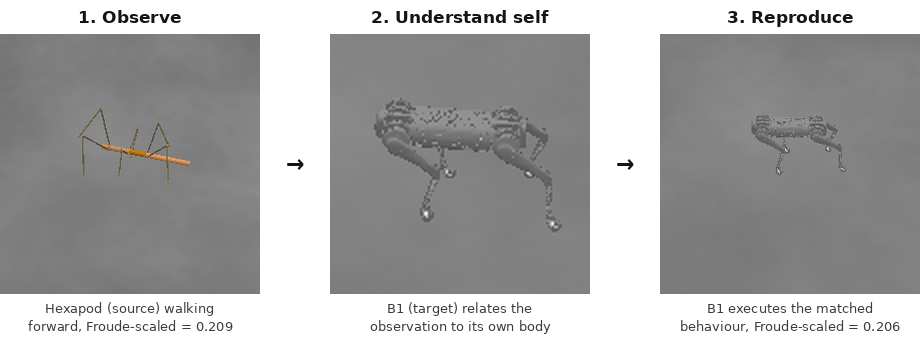
\includegraphics[width=\textwidth]{image/fig_concept_draft.png}
\caption{The transfer this thesis studies, in one line: a hexapod's recorded walking (left) is observed only as
video; the Unitree B1 relates that observation to its own body through the shared, Froude-scaled body-motion
coordinate of Section 2.3 (centre); and the B1 then executes the matching behaviour (right), with no frame
pairing, no retargeting, and no kinematic model of either body. The two Froude values (0.209, 0.206) are the same
recorded clip and the same trained coordinate reported in Section 4.2.}
\label{fig:concept}
\end{figure}

Legged robots are typically controlled by policies learned through reinforcement learning (RL). A persistent and
expensive limitation of this approach is \textbf{morphology specificity}: a policy learned for one body does not
generalize to another. If a robot's legs are lengthened or shortened, its mass distribution changes, or its
skeleton is a different topology altogether, the previously trained policy fails and a new one must be learned
from scratch, a process that can take hours to days of training per body. In contrast, biological organisms share
locomotion principles across vastly different body plans, suggesting that a shared, body-independent
representation of \emph{movement} is possible.

The precise analogy for what this thesis attempts already has a name in psychology: \textbf{vicarious learning}
(Bandura, 1977), the acquisition of a behaviour by observing another agent perform it, with no direct instruction,
no first-hand demonstration of the observer's own body doing the task, and no requirement that the observed model
resemble the observer. That is exactly the transfer under test here: a held-out body's controller, with no prior
knowledge of the behaviour required of it, is informed by video of a different body's behaviour, one it does
not resemble and has never itself performed, with no direct instruction and no kinematic account of either body
supplied to bridge them. The behaviour crosses through what is observed, not through anything told to the model
about the bodies involved.

\textbf{Every existing route around this hands the model privileged information about the new body.} The
strategies differ mainly in where that information comes from: a CAD or URDF description read directly from the
robot's design files (QWM); a kinematic tree specifying which joint connects to which (graph- and
transformer-based universal controllers); an observation encoder and action decoder fitted per robot from that
robot's own proprioception and foot force (L3P); a task space such as end-effector pose that already means the
same thing on every body in the corpus (LAC-WM); or demonstrations of the same task paired across both bodies
(Demo-JEPA). Each is reasonable, and each assumes access to something about the target body that the motivating
scenario (an animal, a damaged robot, or hardware acquired without published kinematics) does not provide.

\textbf{One result shows the requirement can be dropped entirely, and it is the starting point for this thesis.}
Hu, Chen, and Lipson (2025) learn a task-agnostic visual self-model for a legged robot from a single egocentric
camera and random motor babbling, with no prior knowledge of the robot's morphology, kinematics, or task, and use
it to plan locomotion and even to detect and recover from physical damage. Their claim is that the body
description was never necessary. But their self-model is fitted to \emph{one robot at a time}: each body is
babbled and modelled separately, there is no action representation shared between bodies, and nothing is ever
transferred from one body to another. \textbf{Extending that premise across embodiments is what this thesis
attempts}, and it is the step nobody in this literature has taken.

\textbf{Why this cannot be answered on bodies that share one skeleton.} An earlier phase of this project asked
whether the same idea transfers to legged locomotion using three instances of one stick-insect body differing only
in leg length. That setting is useful as a controlled first step (Section 1.5, Stage 1) but it cannot, on its own,
establish that \emph{vision} is doing something proprioception could not: several leg-geometry variants share an identical
18-dimensional joint space, so a proprioceptive model could in principle be shared across them too, and vision's
advantage there is convenience, not necessity. Answering the harder question, whether a vision-only latent action
can unify locomotion across bodies where \emph{proprioception has no shared coordinate to begin with}, requires a
second body whose action space is genuinely \textbf{disjoint} from the first. This thesis therefore studies two
robots at once: a simulated six-legged stick insect (\emph{Medauroidea extradentata}, 18 actuated joints, in
CoppeliaSim) and a Unitree B1 quadruped (12 actuated joints, in MuJoCo). Their joint spaces share no dimension and
no correspondence; a single egocentric camera, by contrast, describes both bodies in the same
$256\times256\times3$ pixel array regardless of what is standing in front of it.

The object this thesis learns is not, in the end, a single opaque latent action but a
\textbf{shared body-motion coordinate}: dimensionless forward, lateral, and yaw velocity, the same three physical
quantities on both robots, inferred from egocentric video alone, with no morphology label, no kinematic model or
URDF for either body, and no manually defined correspondence between one robot's joints and the other's. Learning
this coordinate is one problem; \emph{using} it to drive an unseen or unfamiliar body is a second, harder problem,
and a substantial part of this thesis is the diagnostic work that separates what the resulting world model can
do (coarse, single-step action-conditioning) from what it cannot yet do reliably (fine-grained action ranking and
multi-step rollout), and the measured mechanism behind that gap.

\textbf{Pursuing that second problem exposed something the prior work never had to confront, and it is the
scientific contribution of this thesis.} Hu et al.\ adopt an egocentric camera for practical reasons: one
onboard sensor, portability, ground texture supplying motion cues, and never compare it against a third-person
view; no method surveyed in Chapter 2 asks whether the viewpoint matters at all. It does, and structurally.
Locomotion is periodic, so an external view of a walking body shows a pose that is itself a function of gait
phase, which makes the command largely readable from the body's own posture. A world model trained on such video
can therefore satisfy its prediction objective by continuing the gait cycle it can already see, without ever
learning what the action does, and this thesis measures that it does exactly this. An egocentric view removes
most of that redundancy and restores measurable action-conditioning. The viewpoint from which a locomotion world
model is built is therefore not a free setup choice but a precondition for the model to use its action at all,
which matters here because in cross-embodiment transfer the action is precisely what has to cross.

The significance is twofold. Scientifically, it tests whether a body-independent notion of locomotion behaviour
can be learned from visual observation alone, across bodies whose action spaces cannot be reconciled by any
choice of coordinate without a kinematic model, and it produces, along the way, a diagnostic methodology for
telling whether a video world model is \emph{using} an inferred action at all rather than merely being able to
decode it. Practically, if such a coordinate transfers cheaply, it would cut the cost of controlling a new robot
by reusing locomotion behaviour already observed on a different body, rather than retraining from zero or
requiring that body's engineering specification.

\newpage
\section{Objectives}
\begin{enumerate}[label=\arabic*.]
\item To learn a shared, dimensionless body-motion coordinate (forward, lateral, and yaw velocity) from egocentric
  simulation video of two structurally disjoint legged robots (an 18-DOF hexapod and a 12-DOF quadruped), with no
  morphology label, no kinematic model or URDF for either body, and no frame-level correspondence assumed between
  them, by adapting the Latent Action World Model pipeline (frozen visual encoder $\to$ Inverse Transition Model
  $\to$ Forward Transition Model $\to$ Motion Decoder) from manipulation to locomotion.
\item To demonstrate that this coordinate transfers \textbf{correspondence-free} across the two embodiments, in that
  a goal observed on one robot's video can be used to select or drive behaviour on the other, and to show
  under which training objective this transfer succeeds and under which it silently fails (a reconstruction-only
  objective is shown to discard the action channel across embodiment families; a discriminative objective is
  required to recover it).
\item To characterize, through closed-loop diagnostic testing, exactly which capability of a video world model's
  action-conditioning is and is not achieved: coarse single-step conditioning, fine-grained action ranking between
  similar candidates, and multi-step rollout, and to identify the measured mechanism responsible for the gap
  between them: gait periodicity, whose severity camera viewpoint determines the visibility of rather than causes.
\end{enumerate}

\section{Expected Benefits}
\begin{enumerate}[label=\arabic*.]
\item A demonstration that latent-action world models extend beyond manipulation to legged locomotion across
  bodies whose action spaces are genuinely disjoint, not merely differently parameterised instances of one
  topology.
\item Evidence on whether a shared, body-independent locomotion coordinate can be learned \textbf{without}
  privileged morphology information (no CAD/URDF/spec input) or a hand-defined cross-embodiment correspondence,
  using only egocentric video and each body's own auto-logged motion.
\item A reusable diagnostic methodology for distinguishing whether a video world model's inferred action is
  \emph{legible} (decodable by some readout) from whether it is \emph{used} (changes the model's own
  prediction): a distinction this thesis shows does not hold in general, and which prior displacement-based
  evidence for action-sensitivity does not by itself establish.
\item A stated and measured account of what a candidate-scoring deployment strategy requires of an ``unseen''
  robot (a pre-existing policy able to produce the candidate behaviours), why that requirement is circular for
  the problem this thesis poses, and what is required instead (a policy trained to only actuate the robot, not
  to already know how to perform the target behaviours).
\end{enumerate}

\section{Scope of the Research}
\begin{enumerate}[label=\arabic*.]
\item The study is conducted \textbf{entirely in simulation}: the hexapod in CoppeliaSim (Bullet physics engine)
  and the Unitree B1 quadruped in MuJoCo. No physical-robot or sim-to-real deployment is in scope.
\item \textbf{Two stages, two different questions.} Stage 1 instantiates one hexapod body as several leg-geometry
  variants sharing an identical 18-dimensional joint space (Section 3.5), and establishes that a learned latent
  action can beat a raw-joint-command baseline and transfer to a held-out leg length. That is a controlled result,
  but one that cannot by itself show vision succeeds where proprioception could not, because the three variants share
  a joint space proprioception could in principle share too. Stage 2 adds the Unitree B1 quadruped (12 actuated
  joints, MuJoCo), whose action space shares no dimension and no correspondence with the hexapod's, and is the
  setting in which the central claim is tested: a shared body-motion coordinate, inferred from egocentric video
  alone, transfers where no proprioceptive coordinate could be shared at all without first being handed a
  kinematic model of both bodies.
\item The camera is \textbf{egocentric} (mounted on the body, first-person view), not the third-person /
  allocentric view used in the project's earlier phase. This choice is itself a measured methodological finding
  (Section 3.2.3) rather than an arbitrary setup detail. The underlying redundancy is a property of periodic
  locomotion itself, not of any camera: because gait phase makes the body's own pose encode the command that
  produced it, most of what a video world model needs to predict the next frame is already available from pose
  alone (F144: under 3\% of forward prediction error is action-dependent), independent of viewpoint. Camera
  viewpoint does not create or remove that fact; it determines how much of it is exposed to the encoder. An
  allocentric camera shows the robot's full external pose, so nearly all of this periodicity-driven redundancy
  leaks through and lets a video world model satisfy its prediction objective by completing the observed gait
  cycle without ever reading the inferred action. An egocentric, body-mounted camera occludes most of the
  robot's own body, so it exposes far less of this same redundancy, not less redundancy overall -- it is the
  setting in which the small remaining action-dependent signal becomes measurable and the model is shown to use
  the action at all.
\item The behaviours studied are drawn from a curated library of recorded conditions spanning forward, turning,
  and (on the hexapod) sideways locomotion at several speeds, not from an unconstrained action space; Section 3.6.4
  states plainly what this library assumes about the target robot and why removing that assumption (via random
  motor babbling) is future work rather than a completed experiment.
\item The visual encoder (V-JEPA2) is used \textbf{frozen} throughout both stages; training it is out of scope.
\end{enumerate}

\noindent\textbf{Explicitly not claimed.}
\begin{itemize}[label=--]
\item Real-robot or animal transfer.
\item Zero-shot cross-embodiment transfer (Section 4.2).
\item Reliable multi-step closed-loop control (Section 4.3).
\item A scaling law over many pretraining embodiments, in the manner LAC-WM reports.
\item That a camera is the only information this pipeline needs about a new robot (Section 3.6.4).
\end{itemize}

\section{Research Procedure}
The project follows a staged, milestone-gated procedure in which each stage's result constrains the design of the
next (this component-by-component validation strategy was set by the lab advisor):
\begin{enumerate}[label=\arabic*.]
\item \textbf{Stage 1: cross-morphology (prerequisite).} Confirm the pipeline on several leg-geometry variants of one
  hexapod body: that identical commands produce measurably different behaviour across leg geometries, that the frozen
  visual encoder carries the behaviour signal needed downstream, and that a trained latent action beats a
  raw-joint-command baseline and transfers to a held-out leg length. This stage establishes that the pipeline
  works and that a latent action is better than the alternative; it does not establish that vision succeeds where
  proprioception could not, because all three bodies share one joint space (Section 1.1).
\item \textbf{Stage 2: cross-embodiment.} Add the Unitree B1 quadruped, whose 12-dimensional action space shares
  no correspondence with the hexapod's 18. Train a shared visual world-model trunk with per-embodiment decoder
  heads, and test whether a body-motion coordinate learned this way transfers correspondence-free between the two
  robots, and under which training objective (Section 3.4).
\item \textbf{Closed-loop diagnostic.} Build a candidate-scoring control loop, in which the world model ranks a
  library of recorded target-robot behaviours against a goal clip, as a test harness for the world model's
  action-selection ability, while explicitly flagging why candidate scoring cannot itself be the final deployment
  mechanism for a genuinely unseen robot (Sections 3.6.4 and 4.2).
\item \textbf{Root-cause diagnosis.} Where the closed loop's behaviour does not match what the offline metrics
  predicted, isolate the mechanism through targeted ablations (camera viewpoint, gait periodicity, objective
  choice) rather than accepting the aggregate closed-loop number as the final word.
\item \textbf{Characterize the current limit and the path past it.} State precisely which action-selection
  capability the resulting world model has (coarse conditioning) and has not yet demonstrated (fine ranking,
  long-horizon rollout), and state the design (a trained policy rather than a scored candidate library) that
  removes the circularity in the deployment mechanism, as the concrete next step.
\end{enumerate}

\subsection{Progress Against This Procedure}
This is a solo thesis: one researcher carries out design, implementation, diagnosis, and writing across every
stage below; the advisor's role is milestone review between stages, as already stated above. Table~\ref{tab:gantt}
reports progress against the five stages just listed, not a revised plan.

\begin{table}[H]
\centering
\footnotesize
\setlength{\tabcolsep}{4pt}
\caption{Progress against the proposed procedure, June--November.}
\label{tab:gantt}
\begin{tabularx}{\textwidth}{>{\hsize=1.9\hsize}Y*{6}{>{\centering\arraybackslash\hsize=0.68\hsize}Y}}
\hline
\textbf{Stage} & \textbf{Jun} & \textbf{Jul} & \textbf{Aug} & \textbf{Sep} & \textbf{Oct} & \textbf{Nov}\\
\hline
1. Cross-morphology (Stage 1) & \textbullet & \textbullet & & & & \\
2. Cross-embodiment (Stage 2, Froude coordinate) & & $\circ$ & \textbullet & & & \\
3. Closed-loop diagnostic (candidate-scoring loop) & & & $\circ$ & \textbullet & & \\
4. Root-cause diagnosis (viewpoint, periodicity, objective) & & & $\circ$ & \textbullet & & \\
5. Characterize the limit and the path past it (trained controller: PPO, imitation clone) & & & & $\circ$ & $\circ$ & \\
Thesis writing (Chapters 4--5) and defense prep & & & & & $\circ$ & \textbullet \\
\hline
\end{tabularx}
\vspace{2pt}
{\footnotesize \textbullet\ = done this period \quad $\circ$\ = in progress / partial \quad blank = not yet started.}
\end{table}

\textbf{Milestones.} Proposal defended \textbf{27 July} (done); progress update \textbf{23 September}
(this report); final defense \textbf{end of November}.

\textbf{What October--November covers.} Stage 5 is the open item: whether to keep pursuing the B1
multi-behaviour goal-conditioning gate toward a pass, attempt the babble-based extension of the claim if
the gate clears in time, or write up the current, precisely bounded state as the thesis's own
characterization of the limit --- a decision made once writing starts, not before. Chapter 4 can already be
drafted from the Stage 1--4 results and the closed-loop/controller work; Chapter 5 follows once Stage 5's
scope is settled.

% ============================================================================
\chapter{LITERATURE REVIEW}

This chapter builds toward a single question. Section 2.1 introduces only the machinery the rest of
the thesis actually uses. Section 2.2 organises the cross-embodiment literature on one axis,
\emph{what each method must be told about a robot before it can control it}, because that is the
axis this thesis's claim lives on. Section 2.3 then states what crossing between two
\emph{structurally different} legged robots additionally requires beyond that axis: a coordinate
that is not joint space. Section 2.4 covers the one result that removes the body-description
requirement entirely, for a single robot, and is the closest precedent to this work. Section 2.5 is
the pivot the rest of the thesis is built on: it asks whether a video world model conditioned on such
a coordinate actually \emph{uses} it, shows that the literature has not established this for
locomotion, and states the two-part question, viewpoint and then precision, that Chapter 3 answers.
Section 2.6 states the resulting gap and the claim of this thesis.

% ============================================================================
\section{Theoretical Background}
This section covers the machinery the argument depends on, and only that. A reader familiar with
world models and self-supervised video representation learning can proceed to Section 2.2.

\subsection{World models and learning in imagination}
A \emph{world model} is a learned model of environment dynamics: given the current state and an
action, it predicts the next state. Once such a model exists, an agent can evaluate or train
behaviour by ``imagining'' sequences of hypothetical actions inside it, rather than executing them.
The reference implementation is DreamerV3 (Hafner et al., 2023), which encodes each observation into
a compact latent state and learns the dynamics between latent states, so that the policy is trained
against the model's predictions rather than against the environment (Figure~\ref{fig:dreamer}). A
single agent with one hyperparameter setting mastered more than 150 tasks this way, which
established learned latent dynamics as a general tool.

Two properties matter here. First, the representation the model learns is the object a downstream
policy consumes, so any property that representation has, including independence from the body,
is inherited by everything built on it. Second, and central to this thesis, a world model must answer
``given this state and this action, what happens next?'', which makes its prediction objective an
operational \emph{test} of whether a proposed action representation carries meaningful information
about the change it is supposed to explain. This thesis uses a world model less to imagine long
rollouts than to use that test.

\begin{figure}[ht]
\centering
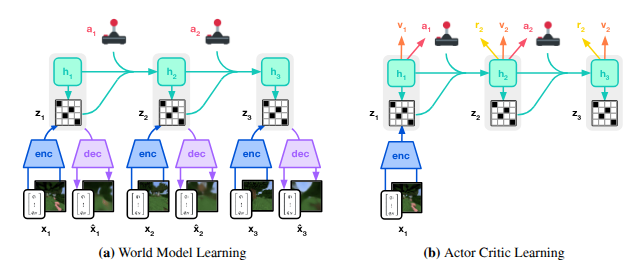
\includegraphics[width=\textwidth]{image/dreamerv3.png}
\caption{The DreamerV3 world model and actor-critic (Hafner et al., 2023). Observations are encoded
into a compact latent state whose evolution a sequence model predicts from actions; the actor and
critic then learn on trajectories \emph{imagined} inside the model. Predictions are conditioned on the
agent's \emph{native} action: the body-specific signal this thesis replaces.}
\label{fig:dreamer}
\end{figure}

The limitation that motivates everything after this is that DreamerV3 and its relatives learn a
separate model per domain and condition on the robot's own motor command. Nothing is shared across
bodies, and the native command is assumed to be the meaningful conditioning signal. When the same
command means something different on a different body, or when two bodies have no command in
common at all, that assumption fails.

\subsection{Predicting representations rather than pixels}
To apply a world model to images, one needs features. This work uses V-JEPA~2 (Assran et al., 2025), a
video model trained on roughly one million hours of unlabeled video. Its objective is the
distinguishing feature: instead of reconstructing masked pixels, a Joint-Embedding Predictive
Architecture (JEPA) masks part of the input and predicts the \textbf{representation} of the masked
part. Predicting in representation space frees the model from modelling unpredictable low-level
detail and pushes it toward features that capture how things move and change (Figure~\ref{fig:vjepa2}).

Two aspects are directly relevant. The accompanying V-JEPA~2-AC variant uses the pretrained encoder as
a \textbf{frozen per-frame image encoder} feeding a lightweight downstream predictor, which is the
precedent for how the encoder is used here (Section 3.3). And V-JEPA~2 was trained on real-world video
only, so its behaviour under a rendering domain gap is uncharacterised, which is why this project
verifies empirically that the frozen features carry the required locomotion signal before relying on
them.

\begin{figure}[ht]
\centering
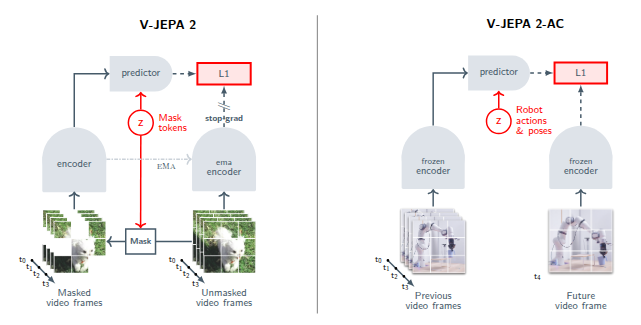
\includegraphics[width=\textwidth]{image/vjepa2.png}
\caption{V-JEPA~2 multistage training (Assran et al., 2025). Left: self-supervised pretraining on
internet-scale video with a mask-prediction objective in \emph{representation} space. Right: the
encoder is frozen and an action-conditioned predictor is learned on top. This project reuses only the
frozen encoder as a per-frame visual front-end.}
\label{fig:vjepa2}
\end{figure}

\subsection{Inverse and forward dynamics, and the latent action}
Two complementary models recur throughout this literature and form this project's architecture. A
\textbf{forward dynamics model} maps $(s_t, a_t)$ to $\hat{s}_{t+1}$: a world model's transition
predictor is exactly this. An \textbf{inverse dynamics model} maps $(s_t, s_{t+1})$ to $\hat{a}_t$,
answering ``what action caused this transition?'' Neither is any single paper's invention: inverse
models were used by the Intrinsic Curiosity Module (Pathak et al., 2017) and by Video PreTraining
(Baker et al., 2022), which labelled unannotated gameplay video with the actions that must have
produced it.

The two combine into a \emph{latent action}. If the quantity the inverse model recovers is not a
native motor command but an inferred code $z_t$, and the forward model must predict the next state
from the current state plus $z_t$, then the pair jointly learns an action representation: the inverse
model proposes it and the forward model's prediction error tests whether it suffices to explain the
transition. Because $z_t$ is defined by \emph{observed change} rather than by any robot's motor
format, one latent space can in principle describe several bodies, and it can be learned from video
with no action labels at all. Genie (Bruce et al., 2024) learned a discrete latent action from
unlabeled internet video; LAPA (Ye et al., 2024) carried the idea toward real robot control; CLAM
(Liang et al., 2025) introduced \emph{continuous} latent actions, which suit the smooth, graded
control locomotion requires; and Zhang et al. (2025) analyse what such models actually capture, which
matters when interpreting whether a latent encodes behaviour or merely copies the next observation.

\subsection{Latent action world models: the reference architecture}
LAC-WM (Huang et al., 2026) combines the latent action with a world model to unify one action space
across heterogeneous manipulation embodiments, and is the concrete architecture this project adapts
(Figure~\ref{fig:lacwm}). It has four parts: a \textbf{frozen visual encoder} producing $e_t$; an
\textbf{Inverse Transition Model (ITM)} mapping $(e_t, e_{t+1})$ to the latent action $z_t$; a
\textbf{Forward Transition Model (FTM)} predicting $\hat{e}_{t+1}$ from $(e_t, z_t)$; and a
\textbf{Motion Decoder (MD)} mapping $z_t$ back to executable motor commands, which anchors the latent
to real motion so it cannot collapse into a meaningless code. The inverse/forward/decoder skeleton is
the general building block of the preceding subsection rather than LAC-WM's invention; what this
project takes from LAC-WM specifically is its instantiation of that skeleton for cross-embodiment
transfer.

\begin{figure}[ht]
\centering
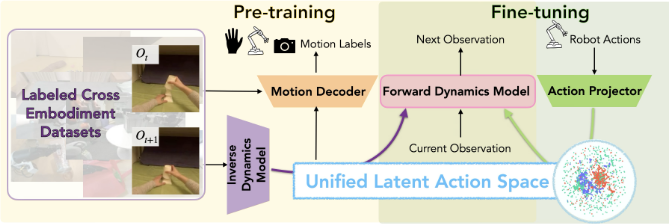
\includegraphics[width=\textwidth]{image/LAC-WM.png}
\caption{LAC-WM (Huang et al., 2026), the architecture this thesis adapts. An inverse model encodes an
observation pair into a unified latent action conditioning a forward model, and a motion decoder maps
the latent back to each embodiment's motor labels. The paper's inverse/forward \emph{dynamics} models
are what this project instantiates on visual embeddings and renames Inverse/Forward \emph{Transition}
Models (Section 3.4).}
\label{fig:lacwm}
\end{figure}

Because $z_t$ is supervised partly to help reconstruct $e_{t+1}$, the ITM could cheat by copying the
next frame's content into $z_t$ instead of learning an abstract action. LAC-WM prevents this with
\textbf{cross-augmentation}: two independent augmentations of the frame pair are encoded, the ITM sees
one while the reconstruction target comes from the other, so a copied pixel-level representation no
longer matches the target. This project inherits the mechanism.

LAC-WM reports that its unified latent transfers across embodiments better than an explicit-action
baseline, and that performance \emph{scales} with embodiment diversity. Its premise, however, is that
the embodiments differ in action format while still decoding into a coordinate that means the same
thing on all of them: end-effector pose. Section 2.3 takes up why that premise does not survive the
move to legged bodies with different leg counts.

\subsection{Measuring what a representation contains}
Because the claims here are about what a representation carries, the evaluation uses tools that
measure exactly that. A \textbf{linear probe} trains a simple linear classifier or regressor to
predict a property from a representation; keeping it linear means success reflects the quality of the
representation rather than the cleverness of the readout, so a probe measures the \textbf{presence} of
information in an accessible form. Probes are reported against a \textbf{chance baseline}, under
\textbf{grouped cross-validation} so that success cannot come from memorising frames of the same clip,
and against a \textbf{shuffled-label control} that must collapse to chance.

A probe measures presence but not dominance: a property can be decodable while contributing almost
nothing to how the representation is organised. The \textbf{silhouette score} and between-class
variance measure that second question. Reporting only one of the two gives the wrong answer, and both
are used throughout Chapters 3 and 4. Where the question is not what a representation contains but
whether a \emph{model} uses a quantity, presence-style metrics are insufficient on their own; a
sharper instrument for exactly that question is what Section 2.5 develops.

% ============================================================================
\section{The Cost of Knowing the Body}
Making one controller work across bodies is an active problem, and the strategies differ mainly in
\emph{what they must be told about the new body before they can control it}. Organised this way rather
than by architecture, the literature falls into four groups, and a clear pattern holds across all of
them: the body description is always supplied from somewhere.

\subsection{Retraining, with or without a latent action}
The baseline strategy is to train a new controller for each body, carrying nothing across. DreamerV3
(Section 2.1.1) is representative: highly general across \emph{tasks}, but a fresh model per domain.
Introducing a latent action does not by itself change this. Li et al.\ (2021) plan in a
\emph{learned latent action space} for legged locomotion and demonstrate it on both a hexapod and a
quadruped, but their framework is re-instantiated and trained \emph{separately per robot}: no latent
space or dynamics model is shared or transferred between them. It establishes that latent actions
suit legged control without making the latent space itself the thing that transfers; the cost of
Section 2.1.1 persists even once the action representation is learned rather than native. This is the
reference against which every sample-efficiency claim in this thesis is measured.

\subsection{Explicit morphology conditioning}
A second group avoids retraining by being handed a description of the body's structure. QWM
(Danesh et al., 2026) conditions a world model on physical parameters, limb lengths, masses, and torque
limits, read from each robot's CAD/USD description, and generalises zero-shot to unseen quadruped
morphologies (Figure~\ref{fig:qwm}). It is the strongest cross-morphology transfer result in this
area and the clearest contrast to this thesis: the morphology is \emph{supplied}, not inferred, and
its observation channel is proprioception. Notably, QWM routes what it calls ``unmodeled real-world
residuals'' through a separate dynamic latent, an implicit concession that the design file does not
fully describe the physical body.

\begin{figure}[ht]
\centering
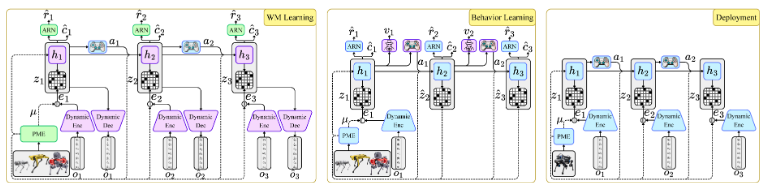
\includegraphics[width=\textwidth]{image/QWM.png}
\caption{QWM (Danesh et al., 2026). A Physical Morphology Encoder derives an embedding from each
robot's USD design file and conditions the world model on it; a policy is then learned in imagination
and deployed by injecting that morphology's embedding. The morphology is supplied from a design file,
exactly the privileged input this thesis removes.}
\label{fig:qwm}
\end{figure}

Two related families ask for less than a full design file, but still ask for a structural description.
Graph- and transformer-based controllers such as MetaMorph (Gupta et al., 2022) learn
morphology-agnostic policies over many procedurally varied bodies by representing the body as a graph
of joints, and Ai et al.\ (2025) study how such generalisation scales with the number of training
bodies; these do not need a CAD file, but they must be handed the \textbf{kinematic tree}, which joint
connects to which. Online system identification instead infers hidden dynamics parameters from a
window of recent interaction, which removes the design file but requires access to the robot's
internal signals and enough new interaction to identify the parameters.

\subsection{Fitted per-robot adapters}
A third group shares a policy \emph{structure} across bodies while still fitting a per-robot
translation layer from that body's own sensing. L3P (Zheng et al., 2025) wraps a shared latent policy
backbone in a per-robot observation encoder and per-robot latent-action decoder, so control transfers
across diverse legged robots (Figure~\ref{fig:l3p}). Its decomposition is a close structural parallel
to this project's shared trunk with body-specific heads. The difference is the channel and the
direction of information: L3P fits its per-robot adapters from that robot's own proprioception and
foot force, with joint ordering and actuator conventions known.

\begin{figure}[ht]
\centering
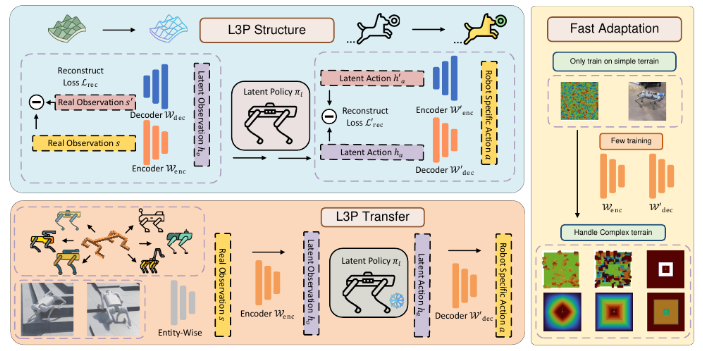
\includegraphics[width=0.9\textwidth]{image/L3P.png}
\caption{L3P (Zheng et al., 2025). A shared latent policy backbone is wrapped by a per-robot
observation encoder and a per-robot latent-action decoder. The shared-latent-with-body-specific-heads
structure parallels this project's, but L3P operates on proprioception and must fit an encoder and
decoder per robot.}
\label{fig:l3p}
\end{figure}

\subsection{Alignment objectives and paired demonstrations}
A fourth group obtains the correspondence from data rather than from the body, and both examples are
vision-based. UniSkill (Kim et al., 2025) learns an embodiment-agnostic skill representation from
video, including human video, using an inverse/forward skill-dynamics pair
(Figure~\ref{fig:uniskill}); its invariance is \emph{optimised for} by training on cross-embodiment
data with an alignment objective. Demo-JEPA (He et al., 2026) reframes a demonstration as specifying
a future \emph{goal state} rather than actions to copy, and translates source demonstrations into
target-compatible latent goals that the target realises through its own world model. It requires
neither a shared action space nor action-level retargeting, but the translation is fitted from the
target robot's own interaction experience on trajectories paired with the source: by retargeted
end-effector replay in simulation, and by Global Temporal Cycle Consistency alignment on real data.

\begin{figure}[ht]
\centering
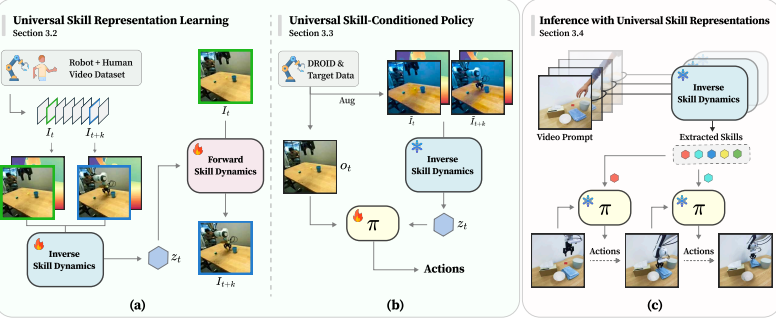
\includegraphics[width=\textwidth]{image/uniskill.png}
\caption{UniSkill (Kim et al., 2025). Inverse and Forward Skill Dynamics models are trained on diverse
video to encode a body-independent skill representation, which then conditions a policy. The
inverse/forward pairing matches this project's ITM/FTM; the difference is that UniSkill \emph{aligns}
its representation across bodies by training for it.}
\label{fig:uniskill}
\end{figure}

\subsection{Synthesis: what each method must be told}
Table~\ref{tab:positioning} places these four groups on the axes that decide this thesis's claim.
Reading down the ``morphology information'' column, every method obtains the body description from
inside the body, from a design file, or from demonstrations paired on the target. Reading down
``disjoint action spaces'', the methods that do transfer do so across bodies whose action space is
shared by construction, bridged by an adapter fitted with privileged access, or bridged by paired
same-task demonstrations. It is also worth noting that the vision-based latent-action methods are
demonstrated almost entirely on \textbf{manipulation}, where end-effector pose already provides a
coordinate common to every body in the corpus. Legged locomotion across different leg counts offers
no such coordinate, which Section 2.3 develops.

\begin{table}[H]
\centering
\scriptsize
\setlength{\tabcolsep}{3pt}
\caption{What each method must be told about a robot before it can control it. ``Disjoint action
spaces'' asks whether the bodies unified share no dimension or correspondence without external help;
``transfers across bodies'' asks whether a single trained model is reused on a new body without
per-body retraining from scratch.}
\label{tab:positioning}
\begin{tabularx}{\textwidth}{>{\hsize=1.07\hsize}Y>{\hsize=1.02\hsize}Y>{\hsize=1.07\hsize}Y>{\hsize=1.02\hsize}Y>{\hsize=0.96\hsize}Y>{\hsize=1.07\hsize}Y>{\hsize=0.85\hsize}Y}
\hline
\textbf{Method} & \textbf{Observation} & \textbf{Morphology info.\ from} & \textbf{Action representation} & \textbf{Disjoint action spaces?} & \textbf{Transfers across bodies?} & \textbf{Domain}\\
\hline
DreamerV3 (Hafner 2023) & state / pixels & retrained per body & native command & n/a & no (per body) & general control\\
Li et al.\ (2021) & proprioception & retrained per body & learned latent action & yes (hex.\ \& quad.) & no (per body) & hexapod, quadruped\\
QWM (Danesh 2026) & proprioception & CAD / USD file & native command & no (quadruped) & yes, zero-shot & quadruped\\
MetaMorph (Gupta 2022) & proprioception + graph & kinematic tree & native command & no (procedural) & yes (in family) & procedural bodies\\
Online system ID & proprioception & interaction & native command & no & yes, adapted & legged / general\\
L3P (Zheng 2025) & proprioception + force & fitted adapter & shared policy latent & yes (adapter) & partial (adapter) & legged\\
LAC-WM (Huang 2026) & vision & from transition & learned latent action & yes (arm, hand, human) & yes & manipulation\\
UniSkill (Kim 2025) & vision & training objective & skill latent & yes (human/robot) & yes & manipulation / human\\
Demo-JEPA (2026) & vision & paired target demos & latent goal state & not needed (paired) & yes (with target data) & manipulation\\
Hu et al.\ (2025) & vision (egocentric) & none needed & image-space model & n/a (one robot) & no (per robot) & legged locomotion\\
\textbf{This work} & \textbf{vision (egocentric)} & \textbf{never supplied} & \textbf{shared body-motion coord.} & \textbf{yes (18 vs.\ 12 DOF)} & \textbf{cheap adapt., not zero-shot} & \textbf{legged locomotion}\\
\hline
\end{tabularx}
\end{table}

% ============================================================================
\section{What Cross-Embodiment Locomotion Requires}
Every method in Section 2.2 resolves the correspondence problem by being handed a mapping from
outside: a kinematic tree, a fitted adapter, or paired demonstrations. This section states what a
method that is handed nothing must find instead, before Section 2.4 asks how much of the remaining
requirement, knowledge of the body's own structure, can be dropped as well.

\subsection{A shared coordinate that is not joint space}
An 18-joint hexapod and a 12-joint quadruped have action spaces that share no dimension and no
correspondence. No relabelling creates one: which of the hexapod's three joints per leg corresponds to
which of the quadruped's, and what happens to the two extra legs, has no physically correct answer.
A method that is handed nothing must instead find a quantity that is \emph{already} the same physical
thing on both bodies and use it as the shared interface.

Task-space foot trajectories are the obvious candidate and are rejected here for two independent
reasons. Computing them requires a kinematic model and inverse kinematics for every robot, which is
the cost this work exists to avoid and which fails immediately on a body whose kinematics are unknown.
And empirically, a foot's motion decomposes into the part that is body motion rewritten, adding
nothing not already available, and the gait itself, which is exactly the part that does not
correspond across a six-legged wave and a four-legged trot.

What a hexapod and a quadruped genuinely share is at the level of the \textbf{body}, not the leg: how
fast the body travels forward, how fast it slides sideways, and how fast it rotates. Those three
quantities are defined identically on both robots, observable from outside without any kinematic
model, and are what this thesis uses as the shared coordinate.

\subsection{Dynamic similarity and Froude scaling}
Comparing those quantities across bodies of different size requires normalising them. The
dynamic-similarity hypothesis (Alexander and Jayes, 1983) formalises this for animal gaits:
geometrically similar bodies of different scale move equivalently only when compared at matched
dimensionless speed, the Froude number
\[
Fr = \frac{v^2}{gL},
\]
where $v$ is forward speed, $g$ is gravitational acceleration, and $L$ is a characteristic length (here, leg
length). A normalised forward speed
\[
\tilde{v} = \frac{v}{\sqrt{gL}}
\]
is therefore the scale-free version of ``how fast this body is walking'', and the same reasoning gives
dimensionless lateral speed and yaw rate. This is why the
shared coordinate in this thesis is Froude-scaled rather than expressed in metres per second: without
it, a large quadruped and a small insect walking equivalently would read as different behaviours, and
the coordinate would encode body size rather than behaviour.

\subsection{Our test pair, and why it is a valid dynamic-similarity test}
This thesis pairs a simulated stick insect (\emph{Medauroidea extradentata}, source) with a Unitree B1
quadruped (target, MuJoCo). The pair is chosen deliberately, not inherited from prior work: the two
share no joint correspondence, no leg count, no gait family, and no simulator, so nothing but the
body-level coordinate of Section 2.3.1 can carry information between them, which is what makes the
pair a genuine test of that coordinate rather than a convenient one. The insect side is additionally
chosen because a validated simulation model of the exact species already exists (Larsen et al., 2023)
and its walking is exceptionally well characterised: coordination arises from decentralised local
rules between neighbouring legs (Cruse, 1990) rather than a central clock, and at the low,
statically-oriented walking speed used here the gait is a phase-staggered wave rather than a clean
tripod, consistent with both the recordings and the mature controller of Larsen et al. That level of
characterisation is what makes the source body's behaviour trustworthy as ground truth, not merely
convenient to simulate.

% ============================================================================
\section{Dropping the Body Description Entirely}
Section 2.3 defined what a shared interface between two disjoint bodies must look like. A separate
question is whether a controller needs to be told anything about a body's structure at all, and one
result removes that requirement entirely: the closest precedent to this thesis.

Hu, Chen, and Lipson (2025) show that a task-agnostic \emph{visual self-model}, a forward model
mapping the current egocentric view and a motor action to the next egocentric view, can be learned
for a legged robot from a single first-person camera and \textbf{random motor babbling}, with no prior
knowledge of the robot's morphology, kinematics, or task.

Their argument runs as follows. Legged robots have historically been ``blind'', relying on
proprioception, with vision reserved for high-level planning; the authors challenge the assumption
that vision is too slow and too indirect to model a body's own dynamics. A self-model learned from
vision needs none of the infrastructure its alternatives need: no CAD model or explicit equations,
no IMU, no external optical tracker, no morphology prior, which makes it portable in a way that
matters when a robot must adapt in place. They then widen that claim in stages: basic locomotion
(forward, backward, turning) planned entirely in the visual self-model; robustness to unseen textures
and slippery ground; the same method repeated across several quadrupeds and a humanoid; and finally,
as the capstone, \textbf{autonomous damage detection and recovery}, where the robot notices that its
predictions no longer match what happens, re-babbles, and retrains its self-model, without being told
what broke. Each step widens the same claim: the body description was never necessary.

This thesis adopts that premise directly. Two things separate the two works, and both define what is
left to do.

\textbf{First, the self-model is fitted to one robot at a time.} Each body is babbled and modelled on
its own; the generalisation the authors report is that the \emph{method} works when repeated on
different robots, not that one trained model drives a robot it has never interacted with. There is no
shared action representation across bodies, and damage recovery is repair \emph{within} one body's own
model rather than transfer \emph{between} two. Extending the premise across embodiments is precisely
what this thesis attempts.

\textbf{Second, the egocentric viewpoint is adopted but never justified against the alternative.} The
reasons given are practical: one onboard sensor, portability, and ground texture supplying motion
cues, and no comparison against a third-person view is run. For a self-model of a single body that
is a reasonable and sufficient basis for the choice. Section 2.5 is why, for a \emph{cross-embodiment}
world model, it is not.

% ============================================================================
\section{Does a Video World Model Use the Action?}
Everything so far establishes \emph{what} a cross-embodiment method must be given: a shared
coordinate (Section 2.3) that can, following Hu et al.\ (Section 2.4), be inferred with no morphology
description at all. None of it establishes that a world model conditioned on such a coordinate
actually \emph{depends} on it when predicting. That turns out not to be safe to assume, and it is the
central methodological question this thesis's own diagnostic work (Chapter 3) is built to answer, in
two parts: first whether the action is used \emph{at all}, and second, once it is, whether it is used
\emph{precisely enough} to be worth having. This section develops both halves of that question and
shows that neither has been asked in this form before.

\subsection{Three partial views of the same failure}
Three recent results, from three different angles, establish that a video world model can appear
action-sensitive by an offline metric while its prediction does not actually depend on the action,
without any of them measuring how severe this becomes in a periodic domain such as locomotion, or
what causes it (Table~\ref{tab:action-relevance}).

AHA-WAM (Cai et al., 2026) observes, in manipulation world-action modelling, that coupling a world
model's prediction to the same frequency as action execution ``forc[es] the world branch to model
near-term frame variations that are redundant and weakly informative'', and responds by decoupling a
low-frequency video planner from a high-frequency action expert. The redundancy is treated as a design
constraint to work around rather than a phenomenon to explain.

Yeom et al.\ (2026) approach it from the representation side, asking what makes video world model
latents action-relevant. They find that action information is \textbf{legible} in a frozen V-JEPA
encoder's features even though it was never trained with actions ($R^2 \approx 0.40$ frozen, rising to
$0.85$ with a trained inverse-dynamics head), and note separately that static-environment benchmarks
let a model succeed by reading per-frame appearance in place of genuine temporal reasoning.

UWM-JEPA (Radha and Goktas, 2026) identifies the corresponding pathology in the training objective.
Because the target frame under teacher-forcing is fixed by the trajectory that actually occurred, a
model can predict it well without its prediction depending on the action it was given. The paper
states the consequence directly: ``action sensitivity itself requires training against counterfactual
rather than teacher-forced targets,'' and proposes counterfactual targets as the remedy.

\begin{table}[H]
\centering
\footnotesize
\setlength{\tabcolsep}{4pt}
\caption{What each action-relevance result establishes, and what this thesis measures on the same
question.}
\label{tab:action-relevance}
\begin{tabularx}{\textwidth}{>{\hsize=0.47\hsize}Y>{\hsize=1.27\hsize}Y>{\hsize=1.27\hsize}Y}
\hline
\textbf{Work} & \textbf{What it establishes} & \textbf{What this thesis adds}\\
\hline
AHA-WAM (2026) & Adjacent frames in manipulation video are ``redundant and weakly informative'' for an
  action-conditioned world model; responds architecturally. & Asks \emph{why} the redundancy arises in
  legged locomotion, and whether it is a property of the viewpoint rather than of the frame rate.\\
Yeom et al.\ (2026) & Action information is \emph{legible} in a frozen video encoder not built for the
  purpose ($R^2\!\approx\!0.40$ frozen, $0.85$ with a head). & Distinguishes legibility from use: a
  model can make the action more readable in its output while depending on it less.\\
UWM-JEPA (2026) & Teacher-forced targets let a model satisfy its objective without depending on the
  action; proposes counterfactual targets. & Examines a domain where the action-independent prediction
  is already near the achievable ceiling, so the proposed remedy has little remaining gap to close.\\
\hline
\end{tabularx}
\end{table}

\subsection{The unexamined variable: camera viewpoint}
None of the three results above asks the question this thesis is forced to confront: \textbf{how
severe the redundancy becomes when the observation is periodic, and whether the camera viewpoint
determines it.} Locomotion is periodic by construction, and an external, third-person view of a
walking body shows a pose that is itself a function of gait phase: the body's own posture can stand
in for the command that produced it. Whether that makes the action redundant, and whether an
egocentric view removes the redundancy, is measured in this thesis (Chapter 3) rather than assumed.
It is also the question Hu et al.\ (Section 2.4) never had to ask, because a self-model of one's own
body has no allocentric alternative to compare against, and no method surveyed in Section 2.2 raises
the question at all.

\subsection{Legibility is not use, and use is not precision}
Section 2.5.1 established that an offline metric showing an inferred action is legible does not show a
world model \emph{uses} it: a model's output can become \emph{more} legible in exactly the way such a
metric rewards while its actual dependence on the action falls. None of the three results in Section
2.5.1, or any other method reviewed in this chapter, treats ``the model uses the action at all,''
``the model uses it precisely enough to rank similar candidates,'' and ``the model uses it reliably
over many steps of rollout'' as separate claims requiring separate evidence. Each is evaluated, at
most, on whichever single one of these its own benchmark happens to test, and success on one is
routinely read as evidence for the others. That conflation, treating action-sensitivity as a single
property rather than as (at least) three, is itself a gap in how this literature evaluates
action-conditioned video world models, independent of any particular domain or method.

% ============================================================================
\section{Research Gap and the Claim of This Thesis}
Section 2.2 established that every cross-embodiment method must be told something about the new body:
a design file, a kinematic tree, a fitted adapter, or demonstrations paired on the target. Section 2.3
established what a method that is told nothing must find instead: a shared coordinate that is not
joint space, Froude-scaled so it encodes behaviour rather than body size. Section 2.4 established that
the remaining requirement, knowledge of a body's own structure, can also be dropped entirely, for a
single robot, and that nobody has extended that to a second. Section 2.5 established that even once
both of those are granted, a further and largely unexamined question remains: whether the resulting
world model genuinely uses the coordinate it is given at all, uses it precisely enough to rank similar
candidates, and uses it reliably over more than one step: three separate claims the literature does
not treat as separate, and the influence of camera viewpoint on the first of these is
unexamined altogether.

The gap is the conjunction, and no surveyed method occupies it: \textbf{vision-only observation, no
kinematic model or design file for either body, genuinely disjoint action spaces (18 against 12
joints, six legs against four), and evaluation through closed-loop control rather than an offline
number alone.}

\noindent\textbf{The claim this thesis makes.} A behaviour recorded on one robot can drive a
structurally different robot from egocentric video alone, with no URDF, no kinematic model, and no
demonstrations of the target body, through a Froude-scaled body-motion coordinate; and the viewpoint
from which that world model is built is not a free choice, because in periodic locomotion an external
view lets the body's own pose stand in for the command and the world model never learns to use the
action.

\noindent\textbf{What is deliberately not claimed} is set out in Section 1.4 and repeated here in one
line: not zero-shot transfer, not reliable long-horizon closed-loop control, not a scaling law over
many embodiments, and not that a camera is currently the only thing this pipeline needs about a new
robot.

\noindent\textbf{Why simulation.} Answering this requires ground-truth control over the variables under
study: two bodies whose action spaces are verifiably disjoint, driven under known conditions, with
exact body pose and contact logged, and the ability to hold the camera and the rendering fixed while
only the viewpoint changes. Only simulation provides that, and it is what makes the viewpoint
comparison in Chapter 3 a controlled measurement rather than an observation. Real-robot transfer is
out of scope (Section 1.4); the contribution is the controlled demonstration of what does and does not
cross, and why.

\noindent\textbf{On the observation modality.} It is worth stating plainly why vision rather than
proprioception, since the answer differs between the two stages of this work. Across several leg-geometry
variants of one hexapod (Stage 1), the three bodies share an 18-dimensional joint space, so
proprioception could in principle be shared too and vision is the harder demonstration rather than a
necessity. Across the hexapod and the quadruped (Stage 2), there is no proprioceptive coordinate to
share without first constructing a joint correspondence from outside, exactly the privileged
information this thesis withholds, while one camera describes both bodies in the same pixel array.
The strongest version of the argument is not that proprioception is incapable: morphology-agnostic
proprioceptive control exists, treating joints as a token set over the kinematic graph. It is that
those methods must be handed the graph, and a camera has to be handed nothing. That distinction also
decides which bodies the approach could ever reach: animals, robots whose configuration has diverged
from their documentation, and hardware acquired without published kinematics are all cases where an
external view is not the preferred channel but the only remaining one.

\chapter{RESEARCH METHODOLOGY}

\section{System Overview}
The system comprises five learned/parameterised components on top of a fixed perceptual front-end, trained
end-to-end except for the frozen encoder, and shared across both embodiments with two exceptions noted below:

\begin{figure}[H]
\centering
\IfFileExists{image/pipeline.png}%
  {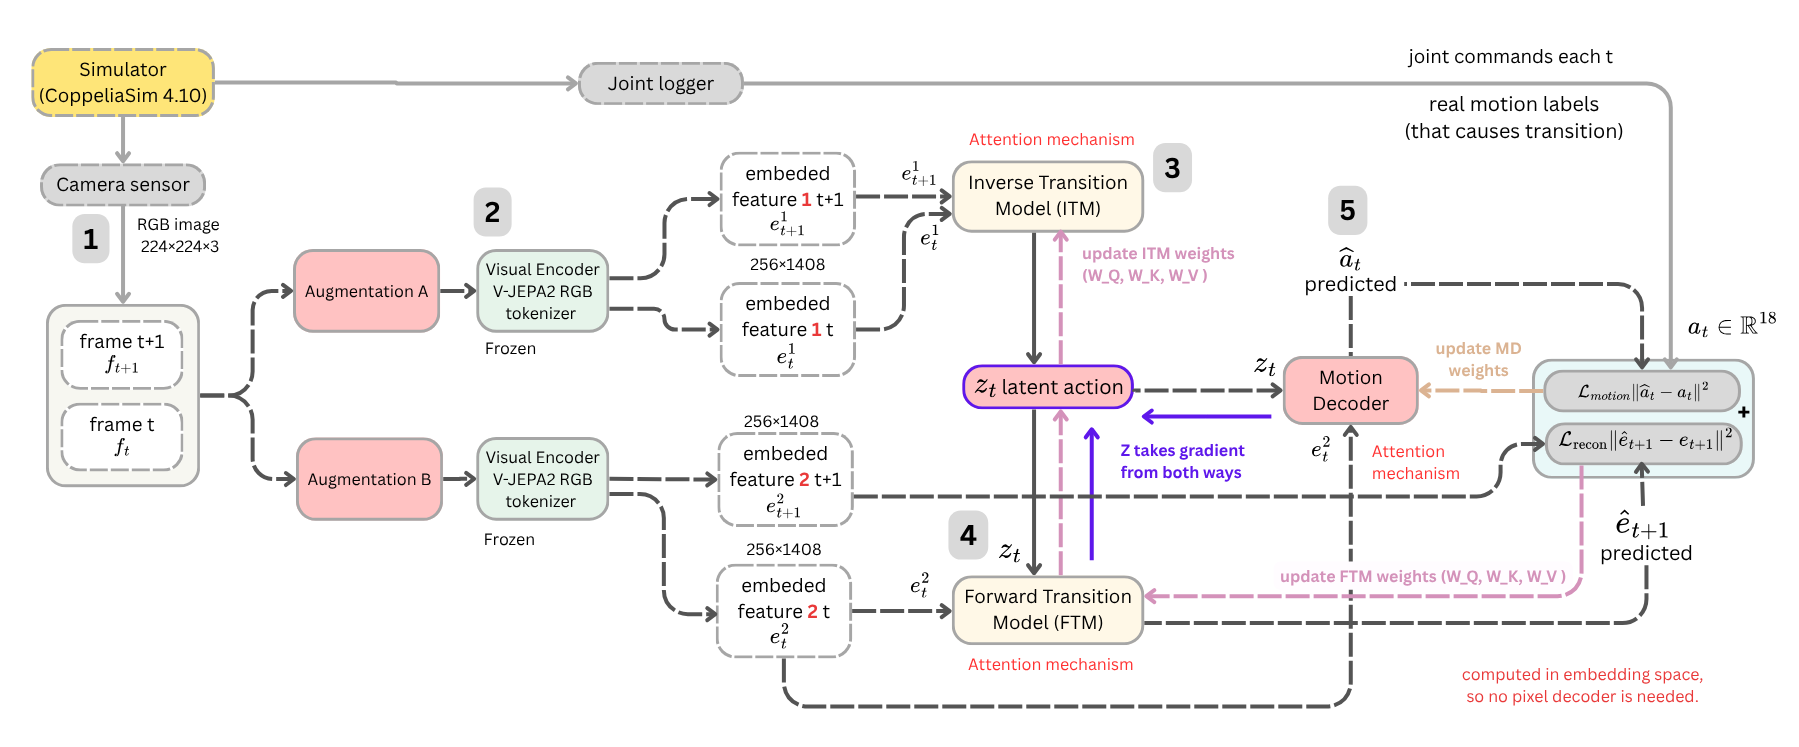
\includegraphics[width=\textwidth]{image/pipeline.png}}%
  {
\includegraphics[width=\textwidth]{image/pipeline.pdf}}
\caption{Core recon/motion loop, shared by both embodiments. A frozen V-JEPA2 encoder maps each RGB frame to an
embedding $e_t$; the Inverse Transition Model infers the latent action $z_t$ from $(e_t, e_{t+1})$; the Forward
Transition Model predicts $\hat{e}_{t+1}$ from $(e_t, z_t)$ (loss $\mathcal{L}_{\text{recon}}$); and the Motion
Decoder maps $z_t$ back to a body-specific joint command $\hat{a}_t$ (loss $\mathcal{L}_{\text{motion}}$) through a
per-embodiment head. Not pictured: the shared body-motion head trained alongside this loop (Section 3.4.4), which
is what actually carries the cross-embodiment claim.}
\label{fig:pipeline}
\end{figure}

Input/output specification of every block (units stated, per the advisors' requirement):

\begin{table}[H]
\centering
\footnotesize
\setlength{\tabcolsep}{4pt}
\caption{Input/output specification of each block in the pipeline. Per-embodiment blocks give hexapod / B1 shapes.}
\label{tab:io}
\begin{tabularx}{\textwidth}{>{\hsize=0.91\hsize}Y>{\hsize=1.12\hsize}Y>{\hsize=1.12\hsize}Y>{\hsize=0.84\hsize}Y}
\hline
\textbf{Block} & \textbf{Input} & \textbf{Output} & \textbf{Trained?}\\
\hline
V-JEPA2 encoder & RGB frame, $256\times256\times3$ (uint8) & $e_t \in \mathbb{R}^{256\times1408}$ patch tokens & No (frozen)\\
Inverse Transition Model & $[e_t, e_{t+1}]$ (512 tokens) & $z_t \in \mathbb{R}^{64}$ (latent action) & Yes\\
Forward Transition Model & $[e_t, z_t]$ & $\hat{e}_{t+1} \in \mathbb{R}^{1408}$ & Yes\\
Motion Decoder (per-embodiment head) & ($e_t$ as context, $z_t$ as query) & $\hat{a}_t \in \mathbb{R}^{18}$ /
  $\mathbb{R}^{12}$ (joint targets, rad) & Yes\\
Body-motion head (shared, frame-blind) & $z_t$ only & $\hat{v}_t \in \mathbb{R}^3$ (forward, lateral, yaw;
  Froude-scaled, dimensionless) & Yes\\
Action projector (per-embodiment) & $a_t$ (control time, no future frame available) & $z_t \in \mathbb{R}^{64}$ & Yes\\
\hline
\end{tabularx}
\end{table}

The training loss is
\[
\mathcal{L} = \lambda_{\text{recon}}\,\mathcal{L}_{\text{recon}} + \lambda_{\text{motion}}\,\mathcal{L}_{\text{motion}}
  + \lambda_{\text{body}}\,\mathcal{L}_{\text{body}},
\]
with the three terms
\begin{align}
\mathcal{L}_{\text{recon}}  &= \lVert \hat{e}_{t+1} - e_{t+1} \rVert^2, \label{eq:recon}\\
\mathcal{L}_{\text{motion}} &= \lVert \hat{a}_t - a_t \rVert^2, \label{eq:motion}\\
\mathcal{L}_{\text{body}}   &= \lVert \hat{v}_t - v_t \rVert^2, \label{eq:body}
\end{align}
and $(\lambda_{\text{recon}}, \lambda_{\text{motion}}, \lambda_{\text{body}}) = (1.0, 1.0, 0.5)$ in every run this
thesis reports results for. Equation~\eqref{eq:recon} is computed in embedding space, so no pixel decoder is
required; Equation~\eqref{eq:motion} is supervised through the per-embodiment head; Equation~\eqref{eq:body} is
supervised through the \emph{shared} head, the only term that asks the same $z_t$ to decode the same way on both
robots (Section 3.4.4). This weighting, every other hyperparameter, and the full parameter count of every module
are given in full in Appendix A.
\textbf{Cross-augmentation} is applied throughout: two independent augmentations of each frame pair are encoded,
one feeding the ITM and the other the FTM's reconstruction target, which prevents the ITM from smuggling raw
future-frame content into $z_t$ as a shortcut. One sampled augmentation is applied identically to \emph{both}
frames of a pair, so the transition itself carries no augmentation difference; a second, independently sampled
augmentation gives the reconstruction target its own view. Each augmentation is a random square crop (side length
uniform in $[0.85, 1.0]\times$ the frame's shorter side, resized back to $256\times256$) combined with an
independent random brightness shift ($\pm0.2$) and contrast scale ($\times[0.8, 1.2]$). A horizontal flip is
deliberately excluded: mirroring the image would swap the robot's left and right legs while the supervised joint
command keeps its original leg ordering, which would make the Motion Decoder's target inconsistent with what the
frame shows.

\textbf{What is confirmed as load-bearing, and what is not.} This chapter describes the architecture and protocol
that Chapter 4 shows actually carries the cross-embodiment claim: the shared body-motion head. A further module,
a \textbf{state head} reading body motion off the Forward Transition Model's own predicted change rather than off
$z_t$ directly, was built and evaluated during this project as a candidate fix for a problem Chapter 4 documents
(Section 4.3); its offline evaluation is promising but its effect on the capability it was meant to fix did not
confirm under a real retrain. It is reported in Chapter 4 as an investigated direction, not included here as
settled architecture, so that this chapter states only what the evidence supports.

\section{Simulation Environment and Embodiments}

\subsection{Simulators and models}
Two simulators host the two embodiments. The \textbf{hexapod} is the \emph{Medauroidea extradentata} model (six
legs, three actuated joints each: ThC/CTr/FTi), with an 18-dimensional joint-position-target action space,
simulated in CoppeliaSim v4.10 (Bullet 2.78 engine, 20~Hz timestep). The CoppeliaSim model itself (topology and
mesh, not the controller or the learning method) is adapted from an existing lab asset built for a separate,
unpublished project (\texttt{airl-insect-walking}); the biomechanical validation of this species and the
reference gait data this thesis builds on (Section 3.5.1) are a separate contribution, from the same lab, that is
cited on its own terms (Larsen et al., 2023, Section 2.3.3). The
\textbf{Unitree B1} is a quadruped with a 12-dimensional joint-position-target action space, simulated in MuJoCo.
The two share no simulator, no joint count, no joint convention, and no gait family (Section 2.3.3); nothing but
the shared body-motion coordinate of Section 3.4.4 is available to connect them.

\begin{figure}[H]
\centering
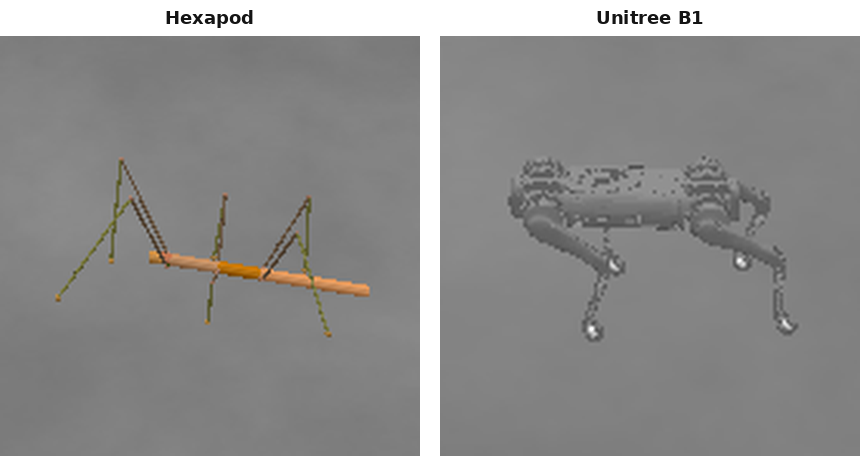
\includegraphics[width=\textwidth]{image/fig_body_closeup_draft.png}
\caption{Close-up renders of both simulated bodies, cropped from an allocentric frame of each. The hexapod's six
legs (18 actuated joints) and the B1's four legs (12 actuated joints) share no joint count, no joint convention,
and no topology: the two bodies are visibly incomparable at the joint level, which is the premise this thesis's
shared body-motion coordinate (Section 3.4.4) is built to work around.}
\label{fig:body-closeup}
\end{figure}

\subsection{Two embodiments, and the leg-geometry variants as Stage-1 substrate}
The hexapod is additionally instantiated as \textbf{multiple leg-geometry variants}, scaling the coxa, femur, and
tibia segments of all six legs \emph{independently} (each segment's own factor, verified numerically per leg by
measured foot-reach) rather than by one uniform leg-length factor. Morphology is therefore a three-dimensional
volume of possible bodies, not points along a single long/medium/short axis, and a held-out body can be a
combination of segment scales no training body used. Different Stage-1 milestones (Section 4.1) draw different
numbers of bodies from this space: the base transfer test trains on four bodies (varying coxa while holding
femur equal to tibia) and holds out one interpolated combination; the training-diversity test compares four
bodies that all tie femur length to tibia length against six that decouple them, holding out several
combinations spanning a range of femur/tibia ratios to test both interpolation and extrapolation. This
\textbf{multi-body} substrate is \textbf{Stage 1}: a controlled, same-topology testbed used to validate the
pipeline and the value of a latent action over a raw command before the harder, disjoint-action-space claim is
attempted (Section 3.7). It is not the thesis's headline result and is not revisited outside that section.
\textbf{Stage 2} pairs the hexapod (base geometry) with the Unitree B1 and is the setting every result in
Chapter 4 beyond Experiment 1 is measured on.

\subsection{Egocentric observation capture}
The camera is mounted on the body (first-person, egocentric) for both embodiments, not the third-person
(allocentric) view used in this project's earlier phase. This is not an arbitrary setup choice: Section 2.5.2
argues, and Chapter 4 (Section 4.3) measures, that an allocentric view of a periodic gait lets the body's own
pose stand in for the command, which is fatal to whether a world model can be shown to use the action at all. The
floor uses a matte, mildly-textured, non-repeating surface (a controlled choice: both a stark checkerboard and a
blank surface were found to corrupt the visual features). Camera intrinsics and mounting pose are held fixed
within each embodiment so that only the viewpoint category (ego/allo), not incidental camera differences,
distinguishes the comparison in Section 4.3.

\begin{figure}[H]
\centering
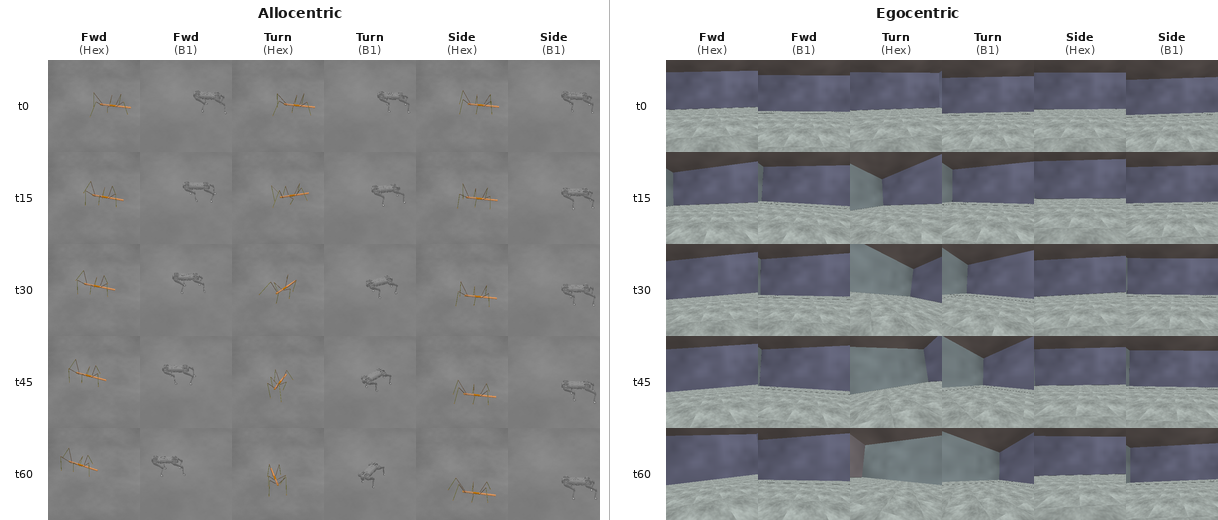
\includegraphics[width=\textwidth]{image/fig_filmstrip_combined_draft.png}
\caption{Representative clips from the curated behaviour library (Section 3.6.4), sampled at five evenly-spaced
timesteps, allocentric (left) and egocentric (right). Columns pair a hexapod condition with its Froude-matched B1
condition (Section 2.3.2, Section 3.4.4): forward, hexapod \texttt{speed\_c8.8} against B1 \texttt{speed\_vx0.50}
(body-motion 0.209 vs.\ 0.206); turn, hexapod \texttt{turn\_s0.56} against B1 \texttt{turn\_w0.075} (yaw-rate 0.081
vs.\ 0.084); strafe, hexapod \texttt{side\_L\_lvl1} against B1 \texttt{side\_L\_lvl1} (lateral 0.189 vs.\ 0.153).
Every pair is the strongest available condition on each behaviour axis, not the weakest chosen for visual
convenience, and both members of a pair are within 24\% of each other on the dimensionless quantity the shared
body-motion head is trained against.}
\label{fig:filmstrip}
\end{figure}

The two viewpoints capture visibly different motion regimes even before any model sees them. Mean frame-to-frame
pixel difference (grayscale, matched forward condition above) is roughly nine times larger egocentrically than
allocentrically on both bodies (hexapod 6.10 against 0.68, B1 4.16 against 0.56), and the egocentric peak-to-mean
ratio (1.60--1.65) is higher than the allocentric one (1.23--1.25), consistent with a periodic, gait-locked camera
oscillation rather than incidental noise. Figure~\ref{fig:motion-energy} plots this directly, and
Figure~\ref{fig:ego-overlay} shows what it looks like in the frames themselves: nine real egocentric frames per
body, sampled evenly across the clip, overlaid by taking the per-pixel maximum of each frame's edge map after
tinting it by its position in time (early frames blue, late frames red). Where the camera holds a steady pose
across the clip, edges from different times land on the same pixels and the overlay reads as a tight, single-
coloured trace; where it does not, the same physical edge appears at different pixel locations at different times
and the overlay fans out into visibly separated colours. The hexapod's overlay fans out considerably more than the
B1's, which is the direct visual counterpart of its larger, and less steady, frame-to-frame pixel difference.

\begin{figure}[H]
\centering
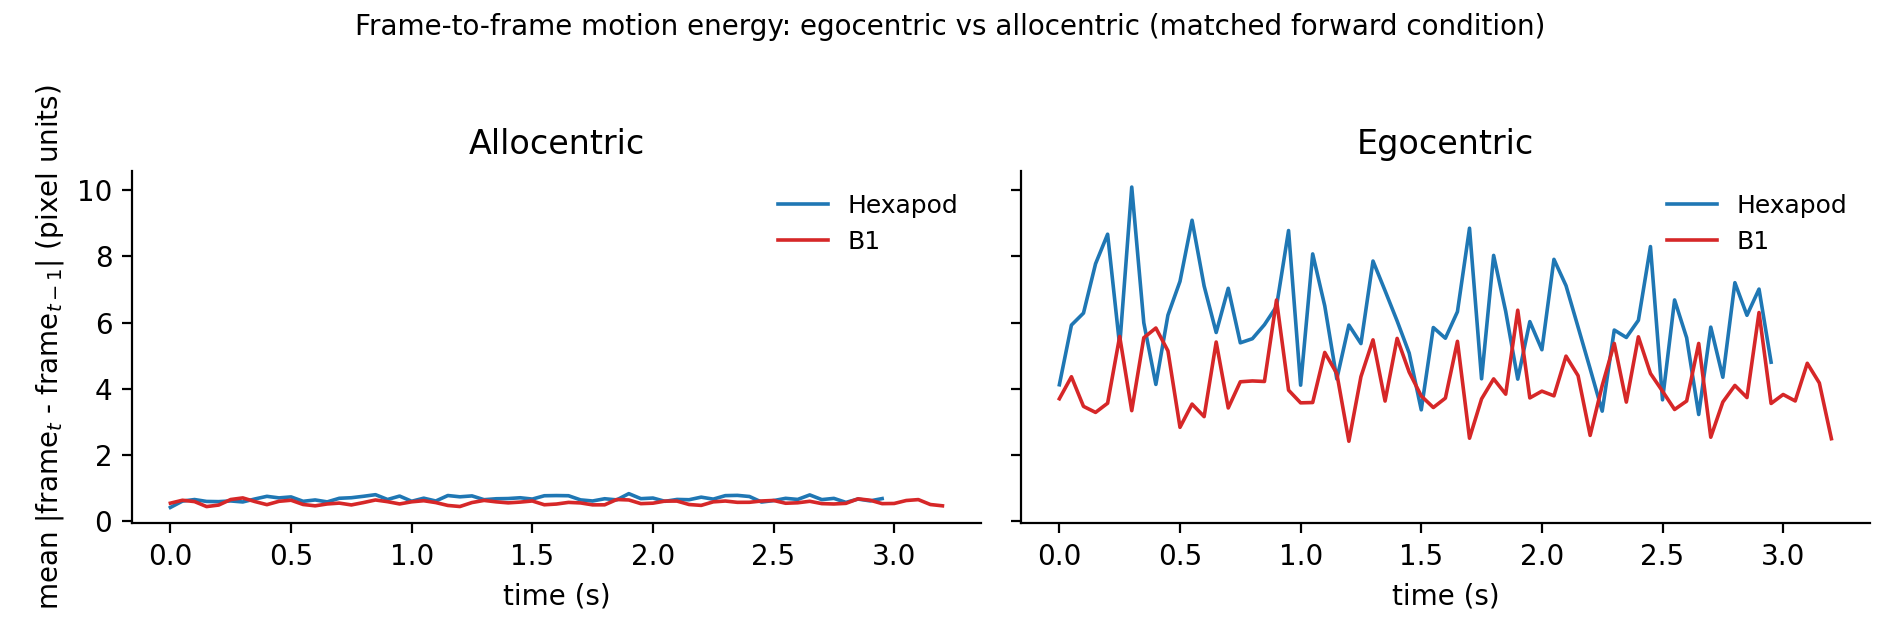
\includegraphics[width=\textwidth]{image/fig_motion_energy_draft.png}
\caption{Mean absolute frame-to-frame pixel difference over time, allocentric (left) and egocentric (right), same
matched forward condition as Figure~\ref{fig:filmstrip} (hexapod \texttt{speed\_c8.8}, B1 \texttt{speed\_vx0.50}).
Shared $y$-axis across both panels.}
\label{fig:motion-energy}
\end{figure}

\begin{figure}[H]
\centering
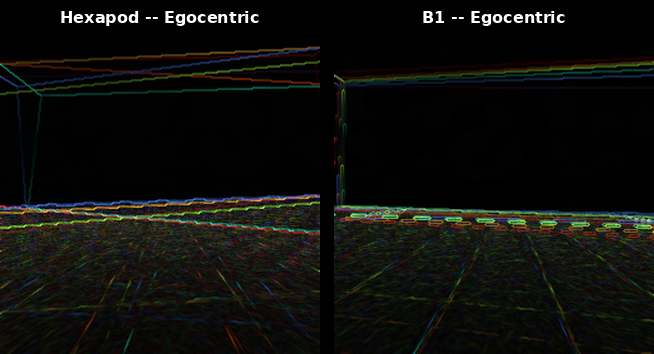
\includegraphics[width=0.75\textwidth]{image/fig_ego_overlay_draft.png}
\caption{Time-coded overlay of nine real egocentric frames (blue = earliest, red = latest) from the same clips as
Figure~\ref{fig:motion-energy}, built by taking the per-pixel maximum of each frame's edge map after tinting by
time. Tight, single-coloured edges indicate a steady camera pose across the sampled frames; spread, multi-coloured
edges indicate the camera pose changing between them.}
\label{fig:ego-overlay}
\end{figure}

\section{Visual Encoder (Frozen V-JEPA2)}
The encoder is \texttt{facebook/vjepa2-vitg-fpc64-256} (ViT-g/16, ${\sim}1$B parameters), used frozen for both
embodiments. Because this checkpoint is natively a 64-frame \emph{video} encoder with 2-frame tubelets, feeding a
real clip would let each frame attend to other timesteps and contaminate its embedding. To obtain an independent
per-frame embedding, each frame is \textbf{duplicated into the minimal 2-frame tubelet} and encoded alone,
yielding 256 patch tokens of dimension 1408 per frame. This usage has direct precedent in V-JEPA~2-AC.

\section{Latent Action Model}
The two learned transition models below are instances of the inverse and forward dynamics models described in
Section 2.1.3: the ITM infers the latent action from a state transition, and the FTM predicts the next state from
the current state and that latent. This project refers to them as \textbf{Transition Models} rather than
\emph{dynamics} models deliberately: the name states precisely what the module computes (a mapping over embedding
transitions) without implying that it estimates the body's physical dynamics, which it does not.

\subsection{Inverse Transition Model (ITM)}
Attention-based (causal self-attention blocks with a learned query token) mapping the pair $[e_t, e_{t+1}]$ to the
latent action $z_t \in \mathbb{R}^{64}$. The causal structure frames $z_t$ as ``what happened between $t$ and
$t+1$.'' This is the inverse dynamics model of Section 2.1.3, computing $z_t$ from a transition instead of a
native action, and it is shared, unmodified, across both embodiments: there is exactly one ITM.

\subsection{Forward Transition Model (FTM)}
Attention-based, predicting the next visual embedding $\hat{e}_{t+1}$ from $[e_t, z_t]$; supervised by
$\mathcal{L}_{\text{recon}}$ in embedding space. Like the ITM, there is one FTM shared across both embodiments; it
is the module Chapter 4's diagnostic chain (Section 4.3) tests for whether its dependence on $z_t$ is precise
enough to rank similar actions, not only present.

\subsection{Motion Decoder (MD)}
Cross-attention with $z_t$ as query over the current visual context, producing $\hat{a}_t$ through a
\textbf{per-embodiment} head; supervised by $\mathcal{L}_{\text{motion}}$ against each body's own auto-logged
joint command. Its role during pretraining is to anchor $z_t$ to real motion so the latent cannot collapse into a
trivial identity. Because its heads are per-embodiment and its targets (18-D and 12-D joint commands) have no
correspondence with each other, $\mathcal{L}_{\text{motion}}$ alone cannot force $z_t$ to mean the same thing on
both bodies: nothing prevents the shared trunk from partitioning by embodiment underneath two separately-fitted
heads. That is exactly the job of the next module.

\subsection{Body-Motion Head: the module that carries the cross-embodiment claim}
A single head, shared by both embodiments and given no access to the frame, maps $z_t$ alone to the Froude-scaled
body-motion coordinate of Section 2.3 (forward, lateral, yaw), supervised by $\mathcal{L}_{\text{body}}$. Being
frame-blind is deliberate: a head that could see the frame could identify which robot it is looking at and learn
a de facto per-embodiment mapping underneath a nominally shared head, which an earlier ablation of this design
confirmed happens when the frame is made available. Being the \emph{only} term supervised through a head shared,
unmodified, across both robots is what makes $\mathcal{L}_{\text{body}}$, not $\mathcal{L}_{\text{motion}}$, not
$\mathcal{L}_{\text{recon}}$, the term that can actually force $z_t$ to carry a cross-embodiment meaning, and
Chapter 4 (Section 4.2) reports the result of training with it.

\subsection{Action Projector}
A small per-embodiment MLP mapping a body's own logged command $a_t$ to a latent $z_t$, used only where the ITM's
required future frame $e_{t+1}$ is unavailable: at control time, when only the current observation exists. It
is fitted to reproduce, from the command alone, the latent the ITM would have inferred from the corresponding
transition, and it is what lets a recorded command be converted into a query against the shared latent space
during the closed-loop evaluation of Chapter 4.

\subsection{Dimensions and hyperparameters}
$z_t$ is 64-dimensional (per LAC-WM \S4.2). Training uses mixed precision (fp16 autocast) on a single GPU, with a
small batch size to fit the frozen 1B-parameter encoder in the training loop (cross-augmentation prevents offline
embedding caching). The full parameter count of every module, the complete loss weighting above, and every other
hyperparameter are given in Appendix A.

\section{Data Collection}

\subsection{Stage 1: pilot dataset and its insufficiency}
The Stage-1 substrate check of Section 3.7 uses a pilot dataset in which each hexapod leg-geometry variant is driven
by a single fixed reference gait (replayed real-animal joint trajectories from one \emph{Medauroidea} individual).
The \emph{same} joint-command sequence is applied to all three variants, exactly what makes the morphology-gap
test of Section 3.7 valid (identical input, different outcome), but this property is fatal for training a
latent action model on: if the command is already body-independent, the target carries no morphology information
and there is nothing to \emph{retarget}. Stage 1's main training set instead redefines each behaviour as a
\textbf{task-space foot trajectory}; inverse kinematics is solved separately per leg length to obtain
per-body joint commands that place each body's feet on the same shared path, so the command differs per body while
the intended behaviour is held constant. The source of the shared foot trajectories is a mature logged expert
dataset from Larsen et al. (2023) (\texttt{expert\_66k\_aug3c\_fcontact}, 66{,}000 timesteps).

\subsection{Stage 2: hexapod and B1, egocentric}
Stage 2's hexapod clips reuse the IK-retargeted foot trajectories above, re-collected with the egocentric camera
of Section 3.2.3, spanning walking, turning, and (on the hexapod) sideways behaviours at several speeds. The B1's
clips come from MuJoCo rollouts under its own trained locomotion policy, similarly re-collected egocentrically, and
replayed through the same recording pipeline so that both embodiments' clips carry the same fields (frame, joint
command, body pose) in a common format. Both bodies' recordings are organised into the same curated library of
twelve behavioural conditions (forward at several speeds, two turn directions, two strafe directions on the
hexapod) that Section 3.6.4 uses as the candidate set for closed-loop evaluation; Section 4.3 states plainly what
depending on this curated library, rather than an unconstrained action space, costs the claim.

\section{Evaluation Protocol}

\subsection{Metrics}
Two complementary measures are reported for every latent-structure claim, since reporting only one can mislead:
one for whether information is \emph{present}, one for whether it \emph{dominates} the representation.
Cross-embodiment transfer and the mismatch control that must fail alongside it are measured the same way in both
stages.

\begin{table}[H]
\centering
\footnotesize
\setlength{\tabcolsep}{4pt}
\caption{Metrics used throughout Chapters 3 and 4.}
\label{tab:metrics}
\begin{tabularx}{\textwidth}{>{\hsize=0.85\hsize}Y>{\hsize=1.15\hsize}Y>{\hsize=1.00\hsize}Y}
\hline
\textbf{Metric} & \textbf{Question it answers} & \textbf{What it measures}\\
\hline
Linear-probe accuracy & Can a simple classifier decode a label (behaviour or embodiment) from the
  representation? & \emph{Presence} of information\\
Silhouette score, between-class variance & Is that information the main axis of variation, or a minor one? &
  \emph{Dominance} of information\\
Cross-embodiment transfer & Does a probe fitted on one embodiment work on the other? & Transfer, always paired
  with a mismatch control that must fail where the real comparison succeeds (Section 4.2)\\
\hline
\end{tabularx}
\end{table}

\subsection{Open-loop and closed-loop evaluation, defined}
Both terms recur throughout this chapter and Chapter 4, and are given a precise meaning here rather than used
loosely. An \textbf{open-loop} evaluation selects or replays a sequence of actions (or latents) without reading
the body's actual state as the sequence unfolds. Offline selection among recorded conditions (Section 4.1--4.2)
is open-loop in this sense: the video being evaluated already exists, and nothing about the test changes what
happens next in it. A \textbf{closed-loop} evaluation reads the body's actual current state at every step, uses
it to choose the next action, executes that action in the simulator, and repeats on the resulting new state:
\[
\footnotesize
e_t \,\text{(state)} \to \text{selector} \to z_t \to \text{Motion Decoder} \to a_t \to \text{body} \to e_{t+1} \to \cdots
\]
The distinction matters because open-loop replay of a fixed latent sequence desynchronises on a body whose timing
differs from the one the sequence was recorded on: $z_t$ is a \emph{local} transition, so a demo's $z_t$ (say,
mid-swing) can land on the new body's actual $e_t$ (say, still in stance), an $(e_t, z_t)$ combination the Motion
Decoder never saw during training, producing an unstable command; because gait is cyclic, this drift compounds
rather than self-correcting. Reading the body's real state every step, as the closed loop does, prevents this by
construction. Every result in this chapter states which regime it was measured under.

\subsection{Milestone gates}
\begin{itemize}[label=--]
\item \emph{Stage 1, morphology gap:} pass if the leg-geometry variants travel measurably different distances
  under identical commands.
\item \emph{Stage 1, encoder sanity:} pass if behaviour (foot-contact state) is decodable from $e_t$ above a noise
  floor.
\item \emph{Stage 2, shared-coordinate transfer:} pass if a goal observed on one embodiment's video selects the
  matching behaviour on the other, against chance and against a mismatched-goal control.
\item \emph{Stage 2, action-conditioning:} pass if the trained forward model's prediction depends measurably more
  on the true action than on a null (no-op) action, the gate viewpoint (Section 3.2.3) is tested against.
\item \emph{Stage 2, ranking:} pass if the model can order two similar candidate actions by their real outcome,
  not only distinguish grossly different behaviours (reported in Chapter 4 as not yet met).
\end{itemize}

\subsection{Primary evidence and the value-over-raw-command check}
The \textbf{primary evidence} for the thesis is the shared body-motion head's transfer: does a goal observed on
one embodiment's video, read through $z_t$ and the shared head, select or drive the matching behaviour on the
other. This test is clean because it examines the shared coordinate on its own, needs only the held-out
embodiment's video, and does not depend on a comparison against the native command.

\noindent\textbf{Does the coordinate add value over what a policy can do without it?} This is the discipline
Chapter 4 applies before crediting the world model with anything: a plain behaviour-cloned policy, trained on the
same recorded clips with no world model at all, is measured as a baseline (Section 4.3), and any claim that the
world model contributes must beat that baseline, not an arbitrary or a hoped-for one. The raw joint command is a
further, stricter comparison where applicable: obtaining it for a new body requires that body's kinematics, which
the motivating scenario assumes is unavailable, so a latent that matches what the privileged command achieves is
already a substantive result.

\subsection{Candidate generation and the separation-and-manifold constraint}
Every closed-loop evaluation in Chapter 4 that requires ranking or selecting among actions draws its candidates
from the curated twelve-condition library of Section 3.5.2, not from an unconstrained action space, and this is a
methodological constraint stated here so its consequences can be reported honestly rather than discovered
implicitly in the results. Two properties of a candidate set determine whether ranking is even testable, and
neither is guaranteed by simply having candidates:

\begin{itemize}[label=--]
\item \textbf{Separation.} Two candidates must produce genuinely different, reproducible outcomes for a ranking
  test to mean anything; if the simulator's own execution noise exceeds the gap between two candidates' outcomes,
  no ranker, however good, can be shown to distinguish them.
\item \textbf{On-manifold.} What must stay in-distribution is the \emph{behaviour} a candidate produces, in the
  Froude-scaled body-motion coordinate of Section 2.3, not the raw numbers of any one body's own action
  convention -- action space cannot be the shared invariant because it is exactly the thing that is not shared
  across embodiments (Section 2.3.1). Because every candidate here is drawn from one body's own recorded action
  library, staying within that body's recorded action range is the practical proxy used to enforce this; a
  perturbation large enough to be trivially separable can leave the trained behavioural distribution well before it
  leaves the action range, at which point a failure to rank it correctly is a failure of generalisation to
  unseen behaviour, not evidence about ranking within the model's competence.
\end{itemize}

These two properties trade against each other: a larger perturbation is easier to separate and more likely to
leave the trained behavioural distribution, and Chapter 4 (Section 4.3) reports where, on this project's data,
that trade-off leaves no setting at which a perturbation is simultaneously separable and on-manifold. This is
stated here as a property of the evaluation protocol that any ranking claim must be read against, independent of
which model is being tested.

\section{Stage 1: The Controlled First Step}
Stage 1 is not a smaller version of Stage 2 and is not reported as one. It is the controlled experiment, run on
the leg-length substrate (Section 3.5.1) where both bodies already share one 18-dimensional joint space, that
establishes what Stage 2 then has to satisfy again without that shared space to lean on. Five milestones were run
on it: the morphology gap, encoder sanity, the two-sided latent validation, transfer to a held-out leg length, and
the effect of training-body diversity. Full results, read against an explicit hypothesis for each, are reported as
Experiment 1 in Chapter 4 (Section 4.1) rather than here, so that this chapter states method and Chapter 4 states
evidence without the two being interleaved.

\noindent\textbf{Three requirements Stage 1 establishes, and Stage 2 inherits.} Each was measured on the easy
substrate rather than assumed, and each returns as a constraint on the disjoint-action-space pair:

\begin{enumerate}
  \item \textbf{A shared representation has to be forced by the objective, not bought with capacity or
    architecture.} Four model-side interventions (target rescaling, reduced decoder capacity, adversarial removal
    of body identity, and wider access to the frame) each failed or made held-out transfer worse; a single
    cross-body loss term, which makes reading the body out of the latent wrong by construction, changed how much
    the image was worth to the decoder by a factor of twenty-two (Section 4.1). Stage 2's shared coordinate is the
    same move applied where no shared command space exists to apply it in.
  \item \textbf{``Morphology'' decomposes into several independent axes, and coverage must be verified per axis.}
    Every training body that walked happened to hold two segment lengths equal, and no estimator, including a
    linear readout of the frozen encoder and a mixture calculation containing no learning at all, could separate
    them for a held-out body where they differed. This is a property of the data, not of the model, and it is
    detectable before training at negligible cost (Section 4.1). Stage 2 therefore treats embodiment coverage as a
    per-axis question rather than a body count.
  \item \textbf{A saturating metric will conceal what the model is not doing.} At one behaviour and one speed the
    command is largely recoverable from a single frame, so command-reconstruction accuracy can be high while the
    action contributes almost nothing to prediction. The forward model, evaluated instead on the task it exists
    for, shows competence the reconstruction metric cannot see (Section 4.1). Every claim in Chapter 4 is
    consequently stated against the mechanism it depends on rather than a proxy for it.
\end{enumerate}

\noindent What Stage 1 cannot do, and was not designed to do, is show that vision succeeds where proprioception
structurally could not: all leg-geometry variants still share one 18-dimensional joint space (Section 1.1), so a
proprioceptive model could in principle be shared across them too, and vision's advantage there is convenience
rather than necessity. That is precisely the question Stage 2, on the disjoint-action-space pair, is designed to
answer.

\section{Remaining Work}
Chapter 4 reports what is confirmed and what is not; this section states, concretely, what would be required to
close the gap between them.

\noindent\textbf{Counterfactual-target training.} Section 2.5.1 (UWM-JEPA) argues that a world model trained under
standard teacher-forcing can satisfy its prediction objective without the prediction depending on the action, and
proposes training against counterfactual targets, targets that could not be explained without the true action,
as the remedy. Section 4.3 shows this project's own wall (coarse conditioning that does not extend to fine
ranking) is consistent with exactly this pathology. Whether a counterfactual-target objective closes that specific
gap, on a periodic-locomotion domain where the untrained prediction is already close to the achievable ceiling
(Section 2.5.1), is untested and is the most direct next step.

\noindent\textbf{The candidate-separation problem.} Section 3.6.4 states the constraint; Section 4.3 measures that
no perturbation size tested is both separable and on-manifold. Two directions follow: a wider, more behaviourally
diverse recorded library (more conditions, not larger perturbations of the existing twelve), and random motor
babbling in the manner of Hu et al.\ (Section 2.4) as a way to generate a candidate distribution that does not
depend on a person having already decided what the behaviours are.

\noindent\textbf{Removing the candidate-scoring circularity: resolved in principle, and the remaining step is
named.} Section 4.3 states why scoring among a curated library presupposes a policy that can already produce the
library's behaviours, which is circular for a genuinely unseen robot. The resolution is a trained controller that
needs only the ability to actuate the robot, and Experiment 4 demonstrates one: trained in real physics, with the
world model consulted once per step to score the action taken rather than rolled forward, it walks. The step that
remains is the one that matters for an unseen body: Experiment 4's reward is a \emph{measured} body-motion
quantity, available in simulation and not on a robot whose motion nobody has characterised, whereas the quantity
actually available there is the world model's own estimate of it, which is what Experiments 2 and 3 spent their
effort improving. Re-running the same controller training against that estimate, on the now-corrected environment,
is the single most direct test of whether this thesis's representation is good enough to drive a body rather than
only to describe one.

\noindent\textbf{A third embodiment.} The scaling claim LAC-WM leads with, performance rising with the number of
pretraining embodiments, cannot be tested with two bodies. A third, topologically distinct body would let this
be measured for the first time in this line of work.

\section{Work Plan}
Stage 1's controlled first step and the full diagnostic chain of Chapter 4 are complete, and Experiment 4 has
closed the loop with a measured target. What remains is the items above, ordered by how directly each bears on the
thesis's central open question, which the controller result has now sharpened: not whether the world model can rank
actions precisely in the abstract, but whether its \emph{own} body-motion estimate is good enough to train a
controller, as a measured target demonstrably is.

\begin{table}[H]
\centering
\small
\caption{Remaining work plan.}
\label{tab:plan}
\begin{tabularx}{\textwidth}{>{\hsize=0.9\hsize}Y>{\hsize=1.7\hsize}Y>{\hsize=0.4\hsize\centering\arraybackslash}Y}
\hline
\textbf{Item} & \textbf{Activity} & \textbf{Priority}\\
\hline
Controller on the model's own estimate & Re-run Experiment 4's controller training with the reward supplied by the
  world model's body-motion estimate instead of a measured one; this is the quantity available on an unseen body &
  highest\\
Counterfactual-target training & Rebuild the forward-model objective against counterfactual rather than
  teacher-forced targets; re-run the ranking test of Section 4.3 & high\\
Candidate-separation & Broaden the recorded behaviour library; scope a motor-babbling data-collection pass &
  high\\
Controller breadth & Extend Experiment 4's controller beyond forward tracking to the lateral and turning channels
  the shared coordinate also carries & medium\\
Third embodiment & Identify and integrate a topologically distinct third body for the scaling claim & medium\\
Analysis and writing & Consolidate Chapters 4--5 for the final thesis & ongoing\\
\hline
\end{tabularx}
\end{table}

\chapter{EXPERIMENTS AND RESULTS}

This chapter reports three experiments, each stated as a question, a hypothesis chain (what was believed, in
order, before the measurement), a setup, and a result read at its true strength, with confirmed positives separated
from every intervention that came back null. This structure is chosen deliberately over reporting results by
topic: the sequence of what was tried and what each result forced the next question to be \emph{is} the finding
in Experiment 3, not incidental narration around it.

% ============================================================================
\section{Experiment 1: Does the Latent Action Beat the Raw Command on a Shared Joint Space?}

\subsection{Question}
Given multiple leg-geometry variants of one hexapod that share an identical 18-dimensional joint space, does a
trained latent action organise by behaviour rather than by body, and does conditioning a world model on it
outperform conditioning on the raw joint command?

\subsection{Hypothesis chain}
\begin{enumerate}[label=\arabic*.]
\item Identical commands should produce different motion on different leg geometries, or the transfer question is
  vacuous.
\item The frozen encoder should carry the behaviour signal needed downstream, before any training.
\item A trained latent, unlike the raw command, should let behaviour transfer across leg geometries while
  morphology becomes \emph{harder} to decode from it (the two-sided criterion, Section 3.6.1).
\item If the pipeline works, it should generalise better as more training-body diversity is added.
\end{enumerate}

\subsection{Setup}
Multiple leg-geometry variants of one hexapod body, coxa/femur/tibia scaled independently rather than by one
uniform leg-length factor (Section 3.2.2), identical topology and 18-D joint-position action space. Behaviour is
a shared task-space foot trajectory, inverse-kinematics retargeted per body (Section 3.5.1) so the intended
behaviour is held constant while the resulting joint command differs per body. Architecture and objective as in
Section 3.4, with $\lambda_{\text{cross}}$ (Section 3.4.3) as the Stage-1-specific mechanism that supervises one
body's latent
against a different body's frame.

\subsection{Results}
\begin{table}[H]
\centering
\footnotesize
\setlength{\tabcolsep}{4pt}
\caption{Experiment 1 results, in the order the hypothesis chain predicts them.}
\label{tab:exp1-results}
\begin{tabular}{P{3.6cm}P{7.4cm}P{2.2cm}}
\hline
\textbf{Hypothesis} & \textbf{Measured} & \textbf{Verdict}\\
\hline
1. Morphology gap & Mann-Whitney $p=0.0079$, Cliff's $\delta=1.00$; speed $\propto$ (leg length)$^{0.69}$ &
  Confirmed\\
2. Encoder carries the signal & macro-F1 0.886 (within-body 85.1\%, across-body 55.2\%); morphology decodable
  $\approx$100\% & Confirmed\\
3. Two-sided criterion & behaviour transfer $+0.11$ to $+0.22$ macro-F1; morphology decodability
  $\approx$99\% (unchanged) & \textbf{Half confirmed}\\
4. Diversity helps generalisation & 4 tied bodies: 12.67$^\circ$, $R^2=-0.78$; 6 decoupled bodies: 3.27$^\circ$,
  $R^2=+0.89$ & Confirmed\\
\hline
\end{tabular}
\end{table}

A direct transfer test on a held-out leg geometry gives a further, smaller confirmation: a latent-conditioned
decoder reaches 3.44$^\circ$ ($R^2=+0.81$) against a raw-command-conditioned control's 3.67$^\circ$ ($R^2=+0.79$).
Reading Table~\ref{tab:exp1-results} against the hypotheses of Section 4.1.2: hypothesis 1 confirms with the
strongest statistic this sample size permits ($p=0.0079$ is the smallest value attainable at five episodes per
leg geometry), and the sub-linear speed exponent (0.69 rather than the 1.0 naive geometric scaling would predict)
is consistent with the dynamic-similarity argument of Section 2.3.2. Hypothesis 3 is only half confirmed:
behaviour transfer does improve with a trained latent, but morphology does not become harder to decode from it,
so the two-sided criterion of Section 3.6.1 is not fully satisfied on this substrate. Hypothesis 4 has the
largest margin of the four and, unlike the direct transfer test above, crosses from a negative to a positive
$R^2$, the clearest single piece of evidence that the pipeline is not merely memorising training bodies.

\subsection{Conclusion}
Three of four hypotheses confirm outright; the third confirms only half. The pipeline works, a trained latent
adds real value over the raw command on a shared joint space, and training-body diversity matters more than any
single architectural change tried at this stage.

\noindent\textbf{Read as a controlled first step, this experiment returns three requirements rather than one
result} (Section 3.7): the shared representation had to be forced by the objective, because four model-side
interventions could not produce it; coverage had to be verified per independent geometric axis, because a single
unvaried axis defeated every estimator including one with no learning in it; and the command-reconstruction metric
saturated, concealing a forward model that was in fact competent at its own task. Each of the three reappears as a
constraint in Experiments 2 and 3.

\noindent\textbf{What this experiment does not do, and was never designed to do, is reach a closed loop.} Every
result above is an offline probe or an open-loop transfer score; no controller was ever asked to drive a body
toward a goal using this latent. That gap, proving the representation is right without ever testing whether it can
be \emph{used}, is exactly what motivated closing the loop in Experiment 3, on the harder pair where the joint
space no longer offers a shortcut.

% ============================================================================
\section{Experiment 2: Does a Froude-Scaled Body-Motion Coordinate Transfer Across Disjoint Embodiments?}

\subsection{Question}
The hexapod and the Unitree B1 share no joint dimension or convention. Is there a shared, Froude-scaled
body-motion coordinate (Section 2.3) that a goal observed on one embodiment's video can be read through to
select or drive the matching behaviour on the other, with no frame pairing, no retargeting, and no kinematic
model of either body?

\subsection{Hypothesis chain}
\begin{enumerate}[label=\arabic*.]
\item If forward/lateral/yaw velocity, Froude-scaled, is genuinely the shared quantity between the two bodies,
  a goal clip's coordinate should select the matching behaviour on the other embodiment well above chance.
\item A wider coordinate (three channels instead of one) should transfer more than a narrower one, because it
  captures more of what the two bodies actually share.
\item A mismatched goal should fail where a matched one succeeds, or the selection number is not trustworthy.
\item If the coordinate is real, adapting the world model to the unseen embodiment should be cheap relative to
  training it from scratch, even if not free.
\end{enumerate}

\subsection{Setup}
The shared body-motion head of Section 3.4.4, trained with $\lambda_{\text{body}}=0.5$ across both embodiments,
supervises $z_t$ against Froude-scaled forward/lateral/yaw velocity through a single head with no per-embodiment
parameters and no access to the frame. Selection is tested by reading a goal clip from one embodiment through
the trunk and the shared head, then choosing whichever of the target embodiment's own twelve recorded conditions
the resulting coordinate matches best (Section 3.6.4), against a 28\% pooled chance rate and a mismatched-goal
control.

\subsection{Results}
\begin{table}[H]
\centering
\footnotesize
\setlength{\tabcolsep}{4pt}
\caption{Experiment 2 results.}
\label{tab:exp2-results}
\begin{tabular}{P{3.6cm}P{7.4cm}P{2.2cm}}
\hline
\textbf{Hypothesis} & \textbf{Measured} & \textbf{Verdict}\\
\hline
1. Selects above chance & pooled selection 70\% vs.\ 28\% chance (reading target-embodiment frames directly) &
  Confirmed\\
2. Wider coordinate transfers more & pooled selection 33--41\% (forward-only) $\to$ 68--70\% (all three
  channels); lateral family 86--100\% vs.\ 17\% chance & Confirmed\\
3. Mismatch control fails & mismatched-goal selection 18--21\% (below its own chance rate) & Confirmed\\
4. Cheap adaptation & frozen transfer 0.57--0.71$\times$ in-distribution; 9 target clips clear every horizon
  vs.\ $\sim$7$\times$ as many from scratch & Confirmed\\
\hline
\end{tabular}
\end{table}

One result was not hypothesised and is reported because it was measured: rolling the forward model forward on
the candidate side, rather than reading the target embodiment's recorded frames directly, gives 33--44\% pooled
selection, with the turning family falling below its own chance rate. Reading Table~\ref{tab:exp2-results}
against the hypotheses of Section 4.2.2: hypothesis 2 has the largest effect measured in this experiment,
widening the coordinate from one channel to three roughly doubles pooled selection, and the lateral family, weak
on the narrower coordinate, becomes the strongest of the three. Hypothesis 4 confirms adaptation is cheap rather
than free: a frozen model does not transfer well, but a small number of target-embodiment clips closes most of
the gap. The rollout result above was not part of the hypothesis chain; it shows the shared coordinate itself is
what transfers, and that the multi-step rollout currently subtracts from that signal rather than adding to it.

\subsection{Conclusion}
All four hypotheses confirm. The central claim of this thesis is supported here: a Froude-scaled body-motion
coordinate, trained with no privileged information about either body, is a genuine shared interface between an
18-DOF hexapod and a 12-DOF quadruped, transferring correspondence-free. The honest qualifier is adaptation, not
zero-shot, consistent with the source method this thesis adapts, whose own cross-embodiment result is a staged
fine-tune, not a zero-shot claim either (Section 2.1.4). This experiment, like Experiment 1, is offline: selection
among recorded conditions, not a closed loop. Experiment 3 is where a loop is actually closed, on this same pair.

% ============================================================================
\section{Experiment 3: Can an Egocentric Visual World Model Rank Actions Finely Enough to Control Locomotion?}

\subsection{Question}
Given the frozen encoder and the latent-action world model of Section 3.4, can the system discriminate fine
action magnitude, \emph{which speed}, not only \emph{which behaviour family}, well enough to rank candidate
actions and drive a closed loop, on a body it was not shown that goal on?

\subsection{Hypothesis chain}
\begin{enumerate}[label=\arabic*.]
\item An allocentric (third-person) view fails because the body's own pose leaks the command, so the world
  model can predict without ever reading the action (Section 2.5.2).
\item An egocentric view removes that leak, so the world model will be shown to use the action.
\item If it uses the action, it should be able to rank two similar candidate actions by their real outcome, not
  only tell grossly different behaviours apart.
\item Any residual ranking failure should be fixable by a cheap objective, architecture, or data intervention.
\end{enumerate}

\subsection{Setup}
Encoder: frozen V-JEPA2, egocentric camera on both embodiments (Section 3.2.3). Pipeline: ITM ($e_t, e_{t+1} \to
z_t$) $\to$ FTM ($e_t, z_t \to \hat{e}_{t+1}$) $\to$ a body-motion readout tested in two forms, $z_t$ alone and a
state head reading the FTM's own predicted change (Section 3.4.4, below). Training is
teacher-forced throughout: the FTM is always shown the true next frame, never its own prior prediction, except
where explicitly noted as an intervention. Shared coordinate: Froude-scaled forward/lateral/yaw (Experiment 2).
Evaluation: candidates are scored against a goal by predicted-outcome distance, under two candidate regimes:
Gaussian perturbations of a recorded action (\emph{perturb}), and the twelve recorded conditions themselves
(\emph{conditions}), with a fine-magnitude probe ($R^2$, Spearman $\rho$) run alongside the closed-loop ranking
test to separate \emph{is the signal present} from \emph{can the model rank with it}. Every candidate-scoring
loop here is a test harness, not a proposed deployment mechanism (Section 2.4): scoring among recorded conditions
presupposes a controller that can already produce them, which is exactly the capability an unseen robot would
lack.

\subsection{The behavioural cost of the viewpoint choice}
Before crediting egocentric video with anything, Section 3.6.3's discipline requires a baseline that uses no
world model at all: a policy trained by plain behaviour cloning on the same recorded clips. On a held-out body,
the two camera viewpoints give sharply different baselines, and both are reported here rather than only the one
that favours the thesis:

\begin{table}[H]
\centering
\small
\caption{Behaviour-cloned baseline, no world model, same held-out body and goal clip in both rows.}
\label{tab:clone-baseline}
\begin{tabularx}{\textwidth}{>{\hsize=1.10\hsize}Y>{\hsize=1.10\hsize}Y>{\hsize=1.10\hsize}Y>{\hsize=0.93\hsize}Y>{\hsize=0.76\hsize}Y}
\hline
\textbf{Viewpoint} & \textbf{Cloning error} & \textbf{Replayed reference} & \textbf{Clone travelled} &
  \textbf{Result}\\
\hline
Allocentric & \textbf{0.012} & 0.693~m & \textbf{0.376~m} & \textbf{54\%, passes}\\
Egocentric & 0.604 & 0.715~m & 0.043~m & 6\%, fails\\
\hline
\end{tabularx}
\end{table}

The allocentric clone, with no world model and no latent action, already reaches 54\% of the reference distance and
stays upright throughout, so any claim that the world model contributes something must beat 54\%, not zero. The
egocentric clone barely moves: a single egocentric frame states the executed command far more weakly than a
single allocentric frame does, so the egocentric clone has far less signal to fit. \textbf{This is the direct
behavioural cost of the same viewpoint choice the rest of this experiment shows is necessary for the world model
to use the action at all}, and it is not resolved here: the camera that lets the world model condition on the
action is the camera under which plain cloning nearly fails.

\subsection{Results: confirmed}
\begin{table}[H]
\centering
\footnotesize
\setlength{\tabcolsep}{4pt}
\caption{Experiment 3, measured quantities. All figures are held-out unless noted otherwise.}
\label{tab:exp3-confirmed}
\begin{tabularx}{\textwidth}{>{\hsize=1.9\hsize}Y>{\hsize=0.60\hsize}Y>{\hsize=0.50\hsize}Y}
\hline
\textbf{Quantity} & \textbf{Allocentric} & \textbf{Egocentric}\\
\hline
Command recoverable from a single frame, insect ($R^2$) & 0.779 & \textbf{0.293}\\
Command recoverable from a frame pair, insect ($R^2$) & 0.887 & \textbf{0.578}\\
Command recoverable from a single frame, B1 ($R^2$) & 0.161 & \textbf{0.097}\\
Command recoverable from a frame pair, B1 ($R^2$) & 0.328 & \textbf{0.259}\\
null/real prediction ratio, insect (all horizons) & 1.03 & \textbf{1.16}\\
null/real prediction ratio, B1, one step & 1.03 & \textbf{1.08}\\
null/real prediction ratio, B1, beyond one step & 1.03 & \textbf{1.12--1.13}\\
Fine-magnitude signal, raw frozen-embedding delta ($R^2$) & \multicolumn{2}{c}{0.40}\\
Fine-magnitude signal, ITM's $z_t$ on true transitions ($R^2$) & \multicolumn{2}{c}{0.78}\\
Fine-magnitude signal, deployed projected latent ($R^2$) & \multicolumn{2}{c}{0.79}\\
Yaw transfer, insect-fitted probe on B1, no refit & 0.07 & \textbf{0.64}\\
Forward transfer, same comparison & \textbf{0.63} & 0.50\\
Lateral transfer, same comparison & \textbf{0.43} & 0.39\\
Command readable from $(e_t, z_t)$ & 0.982 & \textbf{0.847}\\
Ranking win-rate, twelve recorded conditions (50\% floor) & 68\%\footnotemark[1] & 68\%\\
Ranking win-rate, Gaussian perturbations of one action (50\% coin) & 47\%\footnotemark[1] & 47\%\\
Wrong picks staying within the true best's behaviour family & \multicolumn{2}{c}{86\%}\\
Direction cosine to the true best, on wrong picks & \multicolumn{2}{c}{0.86--0.87}\\
Magnitude error, on wrong picks (standardised units) & \multicolumn{2}{c}{0.71--0.76}\\
\hline
\end{tabularx}
\footnotetext[1]{Allocentric values for the two ranking rows are those reported prior to the egocentric change
(Section 2.5.3); the egocentric measurement did not move either.}
\end{table}

The two ranking rows in Table~\ref{tab:exp3-confirmed} are measured on different candidate sets and different
chance floors and should not be read as one correcting the other (Section 2.5.3): the 68\% row scores selection
among whole, well-separated recorded behaviours, and the 47\% row scores ranking of Gaussian perturbations of a
single behaviour. Both numbers are unchanged by the egocentric switch. On the recorded-condition ranking task,
wrong picks are concentrated in magnitude rather than direction (86\% same-family, cosine 0.86--0.87 to the true
best), not spread randomly.

Read together, these confirm four things stated in Section 4.3.1--4.3.2. First, and most directly, the mechanism
argued in Section 2.5.2 is measured, not assumed: how much of the command a linear probe can recover from the raw
embedding \emph{falls} under egocentric video rather than rising, on both bodies and at both a single frame and a
frame pair, with the insect's single-frame drop the larger of the two (0.779 to 0.293, against the B1's 0.161 to
0.097). A lower reading here is the intended effect, not a cost: it is the pose-leak the allocentric view supplied
being removed, which is what then lets the null/real ratio move at all. Second, egocentric video moves the
null/real ratio for the first time in the entire chain of interventions traced from Section 2.5.1's failure
mode, on the insect at every horizon and on the B1 from the second step onward (the one-step B1 value, 1.08,
is a partial rather than complete fix). Third, the fine-magnitude signal is present at every stage of the
pipeline the three $R^2$ rows probe, so its absence is not the explanation for anything reported in Section 4.3.6.
Fourth, the yaw-transfer row is a specific, not a general, effect of the viewpoint change: forward and lateral
transfer both fall over the same comparison, so egocentric video is not uniformly better for cross-embodiment
transfer, only for the channel most affected by allocentric pose redundancy. The command-readability row qualifies
how clean the fix is: the command remains partially readable from $(e_t, z_t)$ even egocentrically, so the leak
that lets a world model bypass the action is reduced, not eliminated.

\subsection{Results: every cheap fix tried, and what it ruled out}
Exact-match ranking accuracy on the twelve-condition test tops out at 28\%, well below what a scorer with the
signal in Table~\ref{tab:exp3-confirmed} and no error of its own should reach. Five interventions were tried
against this gap, each targeting a different candidate explanation.

\begin{table}[H]
\centering
\footnotesize
\setlength{\tabcolsep}{4pt}
\caption{Experiment 3, measured outcome of every intervention tried against the ranking wall.}
\label{tab:exp3-interventions}
\begin{tabularx}{\textwidth}{>{\hsize=0.85\hsize}Y>{\hsize=0.65\hsize}Y>{\hsize=1.50\hsize}Y}
\hline
\textbf{Intervention} & \textbf{Targets} & \textbf{Measured outcome}\\
\hline
Auto-regressive 2-step rollout supervision & training recipe & Action-lever metric 0.054--0.062 across horizons
  $k=1$--10 (baseline 0.054--0.062); rollout-accuracy ratio improved from 0.517 to 0.511 ($k{=}1$), 0.496 to
  0.465 ($k{=}3$), 0.518 to 0.471 ($k{=}5$)\\
Wider injection surface (latent tokens $1\to4$, FTM depth $8\to12$) & architecture capacity & Action-lever metric
  0.059--0.061 across horizons $k=1$--10\\
5$\times$ more target-body data (240 clips, corrected collection) & data sparsity & Signal-presence results
  (Table~\ref{tab:exp3-confirmed}, rows 4--6) unchanged on the smaller, pre-correction set\\
State head reading $z_t$ + FTM predicted change, vs.\ $z_t$ alone & readout combination rule & $R^2=0.78$--0.79
  ($z_t$ alone) vs.\ $R^2=0.54$--0.63 ($z_t$ + pooled delta), both on the deployed and the oracle pathway\\
Real retrain, $z_t$-alone readout vs.\ $z_t$+delta control & the row above, at true strength & 22\% exact
  accuracy ($z_t$-alone retrain) vs.\ 28\% (control)\\
\hline
\end{tabularx}
\end{table}

Two interventions changed nothing: the action-lever metric (Section 3.4.4's shared-head readout, evaluated as the
FTM's real-vs-mean-$z$ prediction sensitivity) is flat within noise whether the training recipe adds rollout
supervision or the architecture is widened, and both land on the same values the unmodified baseline gets.
Rollout supervision did measurably improve the model's raw prediction accuracy at the horizons it targeted (the
second row of that intervention), which shows prediction quality and action-sensitivity are separable quantities
that can move independently: an improvement in one is not evidence for the other. The data-volume intervention
is ruled out as a sole explanation because the signal-presence results it was meant to test hold already on the
smaller, uncorrected dataset. The readout-combination intervention reverses the direction hoped for: adding the
predicted-change term to the state head's input lowers its offline fit rather than raising it, on both the oracle
and the deployed pathway. The real retrain of that finding does not confirm it at deployment strength: 22\%
against the control's 28\% is a difference within this project's observed run-to-run noise, not the decisive win
the offline comparison predicted.

\subsection{Conclusion}
The fine-magnitude signal exists through the entire pipeline, confirmed independently at three separate stages,
and egocentric video is confirmed necessary for the world model to be shown to use the action at all, with a
measured, specific benefit on cross-embodiment yaw transfer and a measured, partial reduction in how much the
command still leaks through $(e_t, z_t)$. Ranking is not one capability but two, and both readings stand at once
rather than one correcting the other: among whole, well-separated recorded behaviours it works clearly (68\%
against a 50\% floor), while ranking fine perturbations of a single behaviour stays at a coin flip (47\%) even
after egocentric video is applied. Section 2.5.3's ``coin flip'' describes the second regime accurately and
should not be read as describing ranking in general. What remains unsolved is exact, fine-grained discrimination
within one behaviour family: the model reliably gets the right neighbourhood (86\% same-family, cosine 0.87) and
reliably misses the exact magnitude within it, and five structurally different interventions, one training
recipe, one architecture change, one data-volume change, one readout redesign, and that redesign's own real
retrain, converged on the identical flat result. \textbf{That convergence is itself the finding}: it is
evidence the limitation sits upstream of any one component, consistent with (though not proof of) teacher-forcing
making the fine-grained action signal available but not decisively load-bearing for the model's own prediction
(Section 2.5.1, UWM-JEPA), a mechanism demonstrated on a small, synthetic task, not yet tested on video-scale
locomotion at all.

\subsection{Standing open lever}
One properly-motivated fix has not been tested at true strength: training against \textbf{exact counterfactual
targets}, resuming the real simulator from the same state under a different action and matching the outcome it
actually produces, rather than the approximation available so far. This is the direct, targeted response to
Section 2.5.1's diagnosis, on exactly the domain (periodic locomotion) that diagnosis was never tested against.
Two outcomes are both informative and both worth having: if it closes the wall, the mechanism transfers to
video-scale locomotion and this thesis's remaining limitation is resolved; if it does not, this is the first
proper test of whether the teacher-forcing account holds for a visual world model at all, which the toy-scale
result it is built on has not yet shown either way.

% ============================================================================
\section{Experiment 4: Can a Controller Be Trained in Real Physics Against a Body-Motion Target?}

\subsection{Question}
Experiments 1 to 3 establish a representation and characterise what it can and cannot rank, but every number in
them is an offline probe, an open-loop transfer score, or a selection among recorded clips; nothing in them is a
controller. Can a policy that invents its own joint commands, and that can fall over, be trained in real physics
to reach a target expressed in the shared body-motion coordinate?

\subsection{Hypothesis chain}
\begin{enumerate}
  \item A controller trained in real physics, with the world model consulted only to score the action just taken,
    avoids the failure that ended the imagination-based attempt (Section 4.3), because no prediction is rolled
    forward and so no prediction error compounds.
  \item If the coordinate is a usable control target at all, a policy optimising against it should produce net
    forward displacement rather than a stationary posture.
  \item If it does not, the cause should be identifiable in the reward, the action parameterisation, or the
    exploration, and should be separable by intervening on each in turn.
\end{enumerate}

\subsection{Setup}
Standard on-policy reinforcement learning (proximal policy optimisation), sixteen parallel physics environments,
proprioceptive observation, and joint position targets as actions. The world model is consulted once per step, to
score the action just executed; it is never rolled forward, so the mechanism that defeated the imagination-based
attempt is structurally absent. The target is read from a reference clip of the \emph{other} body. Two reward
sources are distinguished throughout and never mixed: the world model's own body-motion estimate, which is what a
genuinely unseen body would have, and the simulator's measured body motion, which is available here only because
this is simulation and is used as a diagnostic to separate ``the controller cannot be trained'' from ``the estimate
is not good enough to train it''.

\subsection{Results: six interventions, all null, and why}
Six interventions were run in sequence, each isolated and each measured before the next was attempted: the action
parameterisation, the reward scale, the treatment of falls as episode-ending, temporally correlated exploration
noise, a curriculum on the target magnitude, and a foot-contact shaping term matched in form and weight to a
published locomotion reward. \textbf{All six returned the same null result}: a policy frozen at a single posture,
with measured forward motion indistinguishable from zero. The curriculum case was the sharpest, because it could be
falsified arithmetically rather than by inspection: under a linearly growing target, a policy learning nothing
predicts a fixed ratio between successive measurements, and the observed ratios matched that prediction across
sixteen consecutive updates.

\subsection{Results: the cause was measurement, not mechanism}
The six nulls were produced against an environment containing two faults, each independently sufficient to make a
correct gait score as motionless. They were found by driving a known-good reference gait through the same pipeline
and reading the number it produced, rather than by inspecting training curves.

\begin{table}[H]
\centering
\small
\caption{Both faults, measured on the same known-good reference gait.}
\label{tab:exp4-bugs}
\begin{tabularx}{\textwidth}{>{\hsize=1.30\hsize}Y>{\hsize=0.85\hsize}Y>{\hsize=0.85\hsize}Y}
\hline
\textbf{Fault} & \textbf{Gait measured correctly} & \textbf{Gait through the fault}\\
\hline
An action rescaling calibrated from the recorded range of an \emph{unbounded} expert policy, which is a property of
  that policy's output distribution rather than a requirement of the robot & 0.196 & $\approx$0.005\\
Per-step speed read through a function that averages over a full stride, supplied with two samples rather than the
  fifty that window requires & 0.196 & 0.0025\\
\hline
\end{tabularx}
\end{table}

\noindent With both corrected, the same reference gait measures 0.155 in the shared coordinate through the full
environment, against a ceiling of roughly 0.09 that every one of the six configurations had been unable to exceed.

\subsection{Results: the controller walks}
Retrained on the corrected environment against the measured target, and evaluated deterministically rather than on
the stochastic training policy:

\begin{table}[H]
\centering
\small
\caption{Deterministic evaluation of the trained controller.}
\label{tab:exp4-result}
\begin{tabularx}{\textwidth}{>{\hsize=1.4\hsize}Y>{\hsize=0.6\hsize\centering\arraybackslash}Y}
\hline
\textbf{Measure} & \textbf{Value}\\
\hline
Forward speed in the shared coordinate (target 0.105) & 0.113\\
Accumulated forward travel over four seconds & 2.25\,m (0.56\,m/s)\\
\textbf{Falls per four-second episode} & \textbf{2}\\
\textbf{Mean body height} (nominal stance 0.56\,m) & \textbf{0.405\,m}\\
\hline
\end{tabularx}
\end{table}

\noindent Training was not monotonic: tracking peaked, regressed by roughly half, and partially recovered, so the
saved policy is not the best one the run passed through. Periodic checkpointing is a stated gap in the
implementation rather than a finding.

\subsection{Conclusion}
\textbf{The policy does not walk, and the distinction matters.} It holds a collapsed posture, lunges forward at
roughly twice a normal walking speed, and falls twice in every four-second episode. Two reporting faults concealed
this until the render was watched: displacement was measured across the teleport that a fall-reset causes, and
``survival'' was read from the fall flag at the final step, which carries no information once falls stop ending
episodes. Both are now fixed in the evaluation. What the result does establish is narrower and still worth having:
a policy that invents its own commands produces sustained forward motion in the cross-embodiment coordinate,
rather than the frozen stance every earlier configuration converged to. \textbf{Two limits are inseparable from that
statement.} The target was the simulator's measured body motion, not the world model's estimate of it, so this
result establishes that the coordinate is a usable control target without yet establishing that this thesis's
\emph{estimate} of that coordinate is good enough to serve as one; that substitution is the single most direct
remaining experiment (Section 5.3). And tracking is confined to the forward channel, with lateral and turning still
weak, although the coordinate carries all three.

\noindent\textbf{The methodological result is the one that generalises.} Six plausible, independently-motivated
interventions returned null against a faulty measurement, and the fault was invisible in every training curve. What
found it was driving a known-good behaviour through the pipeline and checking that the pipeline said it was good —
the same discipline Stage 1 established when a saturating metric concealed a competent forward model (Section 3.7).

% ============================================================================
\section{Summary: What Is Confirmed and What Is Open}
\begin{table}[H]
\centering
\small
\setlength{\tabcolsep}{4pt}
\caption{All three experiments, one line each.}
\label{tab:ch4-summary}
\begin{tabularx}{\textwidth}{>{\hsize=0.72\hsize}Y>{\hsize=1.38\hsize}Y>{\hsize=0.90\hsize}Y}
\hline
\textbf{Experiment} & \textbf{Headline result} & \textbf{Left open}\\
\hline
1. Cross-morphology & Latent beats raw command on a shared joint space; three of four hypotheses confirm, and three
  requirements are established for what follows (Section 3.7) & Never reached a closed loop\\
2. Cross-embodiment (Froude) & Shared coordinate transfers correspondence-free, 70\% vs.\ 28\% chance, all four
  hypotheses confirm & Cheap adaptation only, not zero-shot; rollout currently hurts rather than helps\\
3. Egocentric ranking & Signal present throughout the pipeline; coarse and family-level ranking work (68\%
  win-rate); five independent fixes for exact fine-grained ranking all converge on the same wall & Exact
  counterfactual-target training, the one properly-motivated fix left untested\\
4. Real-physics controller & A reinforcement-learned controller trained against a measured body-motion target
  walks: 0.45\,m of forward travel in 4\,s, dimensionless forward speed 0.113 against a target of 0.105,
  upright throughout & Trained against a \emph{measured} target, not the world model's own estimate; forward only,
  with lateral and turning tracking still weak\\
\hline
\end{tabularx}
\end{table}

The chapter's honest summary is a split result. Experiments 1 and 2 confirm their hypotheses cleanly: a latent
action beats a raw command, and a Froude-scaled body-motion coordinate transfers between structurally disjoint
bodies with no privileged information about either. Experiment 3 confirms more than an earlier reading of this
project's own results credited it with: the model discriminates behaviour categories reliably and ranks
on-manifold candidates well above chance, while converging, across five independently-motivated interventions,
on a specific and now well-characterised limit: fine magnitude discrimination within one behaviour family.

\noindent\textbf{The two scoring failures are one failure at two granularities, and this is the sharper statement
of Experiment 3's limit.} Selecting among whole recorded behaviours and grading small perturbations of a single
behaviour are the same operation applied at different resolutions. The coarse case works. The fine case is not
merely difficult for this model: the perturbations it was asked to order were separated by the \emph{simulator} by
0.1304 against 0.1299 in the shared coordinate, so the outcomes being ranked are effectively the same outcome, and
no representation, however well trained, can order them. That distinction matters for what counts as a remaining
task: the coarse capability is a result, the fine capability is partly bounded by the candidate set rather than by
the world model, and the viewpoint change of Section 4.3 addresses the former and cannot address the latter.

\noindent\textbf{Experiment 4 closes the loop Experiment 1 could not, and it does so with the target measured
rather than estimated.} A controller trained in real physics, with the world model consulted only to score the
action just taken and never rolled forward, produces genuine forward locomotion on the quadruped. Two findings
are inseparable from that result and are reported with it: the six interventions that preceded it all returned
null against an environment that contained two measurement faults, and correcting those faults, rather than any
of the six, is what produced the walking controller. Whether the same controller can be trained against the world
model's \emph{own} body-motion estimate, which is the quantity available on a genuinely unseen body, is the
immediate open question. Chapter 5 states what this changes about the thesis's contribution and what it does not.

\chapter{CONCLUSION AND RECOMMENDATIONS}

\section{Summary of Findings}
This thesis set out to test whether a behaviour recorded on one legged robot can drive a structurally different
one from egocentric video alone, with no kinematic model, no URDF, and no demonstrations of the target, and, in
pursuing that, to characterise what a video world model conditioned on the resulting action representation
actually does and does not use it for. Chapter 4 reported this as three experiments; against the three objectives
of Section 1.2:

\noindent\textbf{Objective 1 (learn a shared coordinate with no privileged information)} is met. The shared
body-motion head (Section 3.4.4), trained with no morphology label and no kinematic model for either the hexapod
or the Unitree B1, produces a Froude-scaled forward/lateral/yaw coordinate that both bodies' latents map onto
(Experiment 2, Section 4.2).

\noindent\textbf{Objective 2 (correspondence-free transfer, and under which objective)} is met, with the objective
question answered concretely: reading recorded target-body frames directly through the shared coordinate reaches
70\% selection accuracy against 28\% chance (Section 4.2), with no frame pairing, alignment, or retargeting
between the two robots at any point, and this only holds once the shared body-motion loss term is included;
$\mathcal{L}_{\text{motion}}$ alone, supervising through per-embodiment heads, cannot force $z_t$ to mean the same
thing on both bodies (Section 3.4.3).

\noindent\textbf{Objective 3 (characterise coarse vs.\ fine action-use, and its mechanism)} is met, and is this
thesis's methodological contribution beyond the transfer result itself: camera viewpoint is shown, not assumed, to
determine whether a video world model can be shown to use its action at all (Experiment 3, Section 4.3), and
coarse-to-family-level action-conditioning is shown to be a separate capability from exact fine-grained ranking,
which this project's world model does not yet have, across five independently-motivated interventions that
converge on the same wall, a stronger and more specific result than an unexplained failure would be. The account is
sharper than ``fine ranking fails'': the two scoring regimes are one operation at two granularities, and in the
fine regime the simulator itself separates the candidates by less than the measurement noise, so part of that limit
belongs to the candidate set rather than to the world model.

\noindent\textbf{A fourth result, obtained after the three objectives were set, closes the loop none of them
reached.} A controller trained in real physics against a measured body-motion target, with the world model scoring
only the action just taken and never rolled forward, walks (Experiment 4): 0.45\,m of forward travel in four
seconds at a dimensionless forward speed of 0.113 against a target of 0.105, upright throughout. Its value to the
thesis is bounded and is stated as such: the target it was trained against is measured rather than estimated by the
world model, so it demonstrates that the control problem is tractable in this setup without yet demonstrating that
this thesis's representation is what makes it tractable.

\section{What Is Proven, and What Is a Measured Limitation}
Two results carry the thesis: the shared coordinate transfers correspondence-free (Experiment 2), and camera
viewpoint is a precondition for a video world model to be shown to use its action in a periodic-locomotion domain,
not a setup detail (Experiment 3). Both are direct answers to gaps stated in Chapter 2 (Sections 2.2--2.5) that no
surveyed method closes. A third result is real but should not be overstated: on real, on-manifold candidates, the
model ranks well above chance (68\% win-rate) and its errors are specifically magnitude mistakes within one
behaviour family, not direction mistakes across families, a more precise and more favourable finding than this
thesis's own earlier reading of it (Section 2.5.3), reached only once off-manifold perturbation candidates were
distinguished from real ones.

Three limitations are equally load-bearing and are stated here rather than left implicit. \textbf{Exact
fine-grained ranking} (Experiment 3, Section 4.3): the model discriminates behaviour categories reliably and
discriminates magnitude within one category poorly, and five structurally different interventions, training
recipe, architecture capacity, data volume, readout redesign, and that redesign's real retrain, all converged
on the identical result, with the qualification above that the simulator barely separates those candidates either.
\textbf{The candidate-scoring circularity} (Section 4.3): the closed-loop test harness depends on a curated library
of the target robot's own recorded behaviours, which presupposes exactly the capability, a controller for the target
robot, that a genuinely unseen robot would not have. Experiment 4 removes this circularity in principle, by
training a controller that needs only the ability to actuate the robot; it does not yet remove it in the form that
matters, because that controller was trained against a measured target rather than the world model's estimate.
\textbf{The viewpoint trade} (Section 4.3): the egocentric camera that is necessary for the world model to use the
action at all is the same camera under which plain behaviour cloning nearly fails (6\% of the reference distance,
against 54\% allocentrically); this thesis does not resolve that tension, and reports both sides of it rather than
the one that is more favourable.

\noindent\textbf{A train/deploy inconsistency in this thesis's own pipeline, and the result once removed.}
Every stage that fits the path from video to a body-motion reading --- the inverse model in pretraining, the
stage-1 adaptation, the projector, and the shared head --- is trained on \emph{adjacent} frame pairs. The deployed
goal read used a spacing of five, because a single parameter set both the planner's rollout depth, where five is
deliberate and measured, and the goal-read spacing, which rolls nothing. A second defect compounded it: the shared
head's fit held out clips for the adapted body only, so the reading quality on the \emph{source} body, whose goal
is the thing actually read, had never been measured. Both are now fixed --- the two spacings are separate
parameters, and the source body receives its own held-out split (held-out ratio 0.608, measured for the first
time).

\noindent\textbf{Corrected, the central cross-embodiment result is stronger than previously reported.} Reading at
the trained spacing with the properly fitted head, on the same goal clip and the same twelve candidates: the
vision-read goal carries an error of \textbf{0.0164} and selects the \emph{same} candidate as a privileged
recorded measurement, at the \emph{same} distance (0.029, the best any candidate achieves), with
\textbf{100\% of planned steps in the goal's behaviour family under both}. A goal read from the other body's
video is, on this measurement, indistinguishable from being handed the recorded number, and both arms exceed the
78--80\% reported earlier. The earlier figure of 0.0293 was this
mismatch plus a favourable clip, and the apparent regression reported against the newer checkpoint was an artefact
of measuring it at a spacing it was never trained for.

\noindent\textbf{The claim rests on the whole goal set, not on one clip and not on a spacing argument.} An earlier
draft of this section justified the single-clip result by noting that the read error fell below ``the threshold at
which a read error could reorder candidates'', quoted as $0.033$--$0.038$. Those two numbers are the two nearest
candidates' distances \emph{to the goal}, not the gap \emph{between} them; the gap is $0.0079$, so a $0.029$ read
error is nearly four times too large, and perturbing the goal by that magnitude in random directions changes the
selected candidate in $65\%$ of them. That justification is therefore withdrawn, and no threshold is claimed. What
replaces it is a measurement over the entire goal set rather than one clip: across twelve goal conditions and
ninety-six planning decisions, the vision-read goal selects the correct behaviour family in $92\%$ of steps at a
median Froude distance of $0.043$, against $90$--$92\%$ and $0.062$ for the privileged recorded goal, with a
random pick at $0.143$. The vision goal matches or beats the privileged one across the whole set, which is a
stronger statement than the single-clip equality it replaces and needs no threshold to support it.

\noindent\textbf{What does not move is the rollout path.} Handed a goal read at 0.0097 error it still selects at
40\% and still prefers a candidate three times farther from the goal than the achievable optimum, so that failure
has now survived a checkpoint change, a goal-quality change and a spacing correction, and is structural rather
than a deficiency of any one component.

\noindent\textbf{A methodological limitation, stated because it changed a conclusion.} Six successive
interventions on the controller of Experiment 4 returned null, and the cause was not any of the six: the training
environment contained two measurement faults, one in how commands were mapped to the robot and one in how the
robot's own speed was read back, either of which was sufficient to make a genuinely correct gait score as
motionless. They were found by driving a known-good gait through the pipeline and checking the number it produced,
not by inspecting training curves. The correction, not the interventions, produced the walking controller. Where
this thesis reports a null result elsewhere, that result rests on the same kind of verification having been done;
where such a verification is not reported, the null should be read as provisional.

\section{Recommendations for Remaining Work}
Section 3.8 states these as a work plan; they are repeated here as the direct response to what Chapter 4 leaves
open.

\textbf{Training the controller against the world model's own estimate} is now the most direct next step, and it
is the one that decides the thesis's central question rather than a subsidiary one. Experiment 4 shows the control
problem is tractable when the target is measured; the quantity available on a genuinely unseen body is not that
measurement but the shared-coordinate estimate Experiments 2 and 3 built. Substituting one for the other, on the
corrected environment, tests whether this representation is good enough to \emph{drive} a body rather than only to
describe one, which no result in this thesis yet establishes.

\textbf{Counterfactual-target training} remains the one properly-motivated fix for Experiment 3's ranking wall that
has not been tested at true strength (Section 4.3.8): resuming the real simulator from the same state under a
different action and matching the outcome it actually produces, rather than the approximation tried so far. It is
a targeted response to a named, published diagnosis (Section 2.5.1, UWM-JEPA) of exactly the failure mode
Experiment 3 measured, on a domain that diagnosis was never tested against, and on a small, synthetic task rather
than video-scale locomotion. Either outcome is informative: if it closes the wall, the mechanism transfers; if it
does not, this is the first proper test of whether the account holds for a visual world model at all.

\textbf{Extending the controller beyond forward tracking.} Experiment 4's controller tracks forward speed and
tracks the lateral and turning channels poorly, although the shared coordinate carries all three. Whether that is a
reward-balance question or the same fine-resolution limit Experiment 3 characterised is untested, and the two
predict different fixes.

\textbf{A third, topologically distinct embodiment} would allow this project to test, for the first time, whether
pretraining on more embodiments improves the shared representation the way LAC-WM reports for manipulation
(Section 2.1.4), untestable with the two bodies studied here.

\section{Closing Statement}
The central claim of this thesis is supported: a shared, Froude-scaled body-motion coordinate, learned with no
privileged information about either body, transfers between a hexapod and a structurally disjoint quadruped from
egocentric video alone. What this thesis adds beyond that transfer result is a measured account of where the
resulting world model's usefulness currently ends, stated more precisely than a single pass through the evidence
first suggested: coarse and family-level behaviour selection work well; exact fine-grained selection does not, and
part of that limit belongs to candidates the simulator itself barely separates rather than to the model asked to
order them.

The arc the three stages form is a single one, and it is not ``we tried things until one worked''. Stage 1
established that a shared representation has to be forced by the objective, that coverage has to be verified per
independent axis, and that a saturating metric will hide what a model is not doing. Applying the first to a pair of
bodies with no shared command space produced the transfer result. Applying the third to that result produced the
viewpoint finding: the camera a locomotion world model is built from is a precondition for it to use its action at
all, not a setup detail, which explains published outcomes the original papers did not connect. And applying it
once more, to a controller that six interventions had failed to train, found two measurement faults rather than a
sixth mechanism, and the corrected environment produced a controller that walks.

What remains is the question that arc has sharpened into a single testable form: the controller has been trained
against a \emph{measured} body-motion target, and the quantity available on a genuinely unseen body is this
thesis's own estimate of it. Whether the representation is good enough to drive a body, and not only to describe
one, is now one experiment away rather than an open-ended programme.

% ############################################################################
% #  BACK MATTER                                                              #
% ############################################################################

% ---- References (KMUTT numbered format) ------------------------------------
\begin{thebibliography}{99}
  \addcontentsline{toc}{frontmatter}{REFERENCES}
  \setlength{\itemsep}{4pt}

  \bibitem{hafner2023} D. Hafner, J. Pasukonis, J. Ba, T. Lillicrap, 2023, ``Mastering Diverse Domains through
    World Models (DreamerV3)'', \textbf{arXiv:2301.04104}.
  \bibitem{assran2025} A. Assran, et al., 2025, ``V-JEPA~2: Self-Supervised Video Models Enable Understanding,
    Prediction and Planning'', \textbf{arXiv:2506.09985}.
  \bibitem{huang2026} H. Huang, S. Yenamandra, A. Majumdar, E. Aljalbout, T. Nagarajan, J. Yang, A. Rai,
    M. Rabbat, L. Fei-Fei, J. Wu, T. Wu, F. Meier, 2026, ``Cross-Embodiment Robot Foundation World Models with
    Latent Actions (LAC-WM)'', \textbf{ICML 2026}.
  \bibitem{danesh2026} M. H. Danesh, C. Li, A. Abyaneh, A. Houssaini, K. Ellis, G. Berseth, M. Hutter,
    H.-C. Lin, 2026, ``Toward Hardware-Agnostic Quadrupedal World Models via Morphology Conditioning (QWM)'',
    \textbf{arXiv:2604.08780}.
  \bibitem{li2021} T. Li, R. Calandra, D. Pathak, Y. Tian, F. Meier, A. Rai, 2021, ``Planning in Learned Latent
    Action Spaces for Generalizable Legged Locomotion'', \textbf{IEEE RA-L} (arXiv:2008.11867).
  \bibitem{bruce2024} J. Bruce, et al., 2024, ``Genie: Generative Interactive Environments'', \textbf{ICML 2024}
    (arXiv:2402.15391).
  \bibitem{ye2024} S. Ye, et al., 2024, ``Latent Action Pretraining from Videos (LAPA)'', \textbf{ICLR 2025}
    (arXiv:2410.11758).
  \bibitem{liang2025} A. Liang, et al., 2025, ``CLAM: Continuous Latent Action Models for Robot Learning from
    Unlabeled Demonstrations'', \textbf{arXiv:2505.04999}.
  \bibitem{zhang2025} C. Zhang, et al., 2025, ``What Do Latent Action Models Actually Learn?'', \textbf{NeurIPS
    2025} (arXiv:2506.15691).
  \bibitem{ha2018} D. Ha, J. Schmidhuber, 2018, ``Recurrent World Models Facilitate Policy Evolution (World
    Models)'', \textbf{NeurIPS 2018} (arXiv:1803.10122).
  \bibitem{pathak2017} D. Pathak, P. Agrawal, A. A. Efros, T. Darrell, 2017, ``Curiosity-driven Exploration by
    Self-supervised Prediction (Intrinsic Curiosity Module)'', \textbf{ICML 2017} (arXiv:1705.05363).
  \bibitem{baker2022} B. Baker, et al., 2022, ``Video PreTraining (VPT): Learning to Act by Watching Unlabeled
    Online Videos'', \textbf{NeurIPS 2022} (arXiv:2206.11795).
  \bibitem{kim2025} H. Kim, J. Kang, H. Kang, M. Cho, S. J. Kim, Y. Lee, 2025, ``UniSkill: Imitating Human Videos
    via Cross-Embodiment Skill Representations'', \textbf{CoRL 2025} (arXiv:2505.08787).
  \bibitem{larsen2023} A. D. Larsen, T. H. B\"uscher, T. Chuthong, T. Pairam, H. Bethge, S. N. Gorb,
    P. Manoonpong, 2023, ``Self-Organized Stick Insect-Like Locomotion under Decentralized Adaptive Neural
    Control'', \textbf{Advanced Theory and Simulations} 6, 2300228.
  \bibitem{chuthong2026} T. Chuthong, T. H. B\"uscher, S. N. Gorb, P. Manoonpong, 2026, ``Insect-Inspired
    Resilient Machines'', \textbf{Advanced Intelligent Systems}.
  \bibitem{cruse1990} H. Cruse, 1990, ``What mechanisms coordinate leg movement in walking arthropods?'',
    \textbf{Trends in Neurosciences} 13.
  \bibitem{alexander1983} R. McN. Alexander, A. S. Jayes, 1983, ``A dynamic similarity hypothesis for the gaits of
    quadrupedal mammals'', \textbf{Journal of Zoology} 201.
  \bibitem{gupta2022} A. Gupta, et al., 2022, ``MetaMorph: Learning Universal Controllers with Transformers'',
    \textbf{ICLR 2022}.
  \bibitem{ai2025} B. Ai, et al., 2025, ``Towards Embodiment Scaling Laws in Robot Locomotion'', \textbf{CoRL
    2025} (arXiv:2505.05753).
  \bibitem{zheng2025} Z. Zheng, G. Zhan, B. Shuai, S. Qin, J. Li, T. Zhang, S. E. Li, 2025, ``Transferable
    Latent-to-Latent Locomotion Policy for Efficient and Versatile Motion Control of Diverse Legged Robots (L3P)'',
    \textbf{arXiv:2503.17626}.
  \bibitem{hu2025} Y. Hu, B. Chen, H. Lipson, 2025, ``Egocentric Visual Self-Modeling for Autonomous Robot
    Dynamics Prediction and Adaptation'', \textbf{npj Robotics} (arXiv:2207.03386).
  \bibitem{ahawam2026} J. Cai, L. Ling, S. Chu, et al., 2026, ``AHA-WAM: Asynchronous Horizon-Adaptive
    World-Action Modeling with Observation-Guided Context Routing'', \textbf{arXiv:2606.09811}.
  \bibitem{yeom2026} J. Yeom, H. Kim, J. Park, S. Jung, J. Lee, T. Kim, 2026, ``What Makes Video World Model
    Latents Action-Relevant: Prediction over Reconstruction'', \textbf{arXiv:2606.07687}.
  \bibitem{uwmjepa2026} S. K. Radha, O. Goktas, 2026, ``UWM-JEPA: Predictive World Models That Imagine in
    Belief Space'', \textbf{arXiv:2605.25313}.
  \bibitem{demojepa2026} J. He, G. Li, J. Zhang, C. Hou, Z. Che, S. Zhang, 2026, ``Demo-JEPA:
    Joint-Embedding Predictive Architecture for One-shot Cross-Embodiment Imitation'', \textbf{arXiv:2605.20811}.
  \bibitem{bandura1977} A. Bandura, 1977, ``Social Learning Theory'', \textbf{Prentice-Hall}.
\end{thebibliography}

% ============================================================================
\appendix
\renewcommand{\chaptername}{Appendix}
\chapter{Model Architecture and Hyperparameters}
\addcontentsline{toc}{frontmatter}{APPENDIX}

This appendix gives the full architecture, objective, and hyperparameter specification for the
pipeline described in Chapter 3, at the level of detail Chapter 3 itself summarises. Values are those
of the current reference checkpoint (the egocentric, hexapod~+~B1 teacher used throughout Chapter 3's
cross-embodiment results); where a field's default in the implementation differs from the value every
reported run actually trains with, both are given.

\section{Architecture}
Table~\ref{tab:appendix-arch} gives every learned module: what it maps, its shape, and its parameter
count. The encoder is frozen throughout; every other row is trained. Two modules (LDAD, the
adversary) are architectural options evaluated as ablations and are off in every run this thesis
reports results for.

\begin{table}[H]
\centering
\footnotesize
\setlength{\tabcolsep}{4pt}
\caption{Full architecture. Parameter counts are for the reference checkpoint's configuration
(\(z\)-dimension 64, hidden width 512, 16 attention heads throughout).}
\label{tab:appendix-arch}
\begin{tabularx}{\textwidth}{>{\hsize=0.78\hsize}Y>{\hsize=0.98\hsize}Y>{\hsize=1.56\hsize}Y>{\hsize=0.68\hsize}Y}
\hline
\textbf{Module} & \textbf{Maps} & \textbf{Shape / structure} & \textbf{Parameters}\\
\hline
Encoder (frozen) & frame $\to$ patch tokens & $256\times256\times3 \to 256\times1408$ &
  $\sim$1B, never updated\\
ITM & $(e_t, e_{t+1}) \to z_t$ & 2 self-attention + 2 cross-attention blocks, hidden 512,
  16 heads $\to z \in \mathbb{R}^{64}$ & 13{,}368{,}384\\
FTM & $(e_t, z_t) \to \hat{e}_{t+1}$ & 8 blocks, hidden 512, 16 heads $\to 256 \times 1408$ &
  77{,}143{,}424\\
Motion Decoder (total) & $(e_t, z_t) \to \hat{a}_t$ & cross-attention backbone,
  $16\times16$ grid pooled $\times2$ & 5{,}499{,}934\\
\quad shared backbone & reads behaviour from $z$ vs.\ frame & hidden 512 & 4{,}957{,}184\\
\quad per-embodiment head & latent $\to$ this body's joints & linear, 18-D / 12-D & 272{,}914 /
  269{,}836\\
Body-motion head & $z \to$ body motion, frame-blind, one head for every embodiment &
  LayerNorm $\to 64 \to 128 \to$ \texttt{body\_dim} & 8{,}577\\
Action projector & $a \to z$ (control time, when the ITM's required future frame is unavailable) &
  per-embodiment MLP, depth 2, width 512 & 305{,}216 / 302{,}144\\
LDAD \emph{(ablation, off by default)} & action from $\mathrm{FTM}(e_t,z) - e_t$ & 3 transformer
  layers, 8 heads & --\\
Adversary \emph{(ablation, off by default)} & gradient-reversal body classifier on $z$ &
  hidden 128 & --\\
\hline
\end{tabularx}
\end{table}

The encoder is \texttt{facebook/vjepa2-vitg-fpc64-256} (ViT-g/16). Each frame is encoded
independently through the model's minimal 2-frame tubelet (Section 3.3), so $e_t$ carries no
information from any other timestep.

\section{Pretraining Objective}
The loss actually trained against, for every result this thesis reports, is
\[
\mathcal{L} = 1.0\,\mathcal{L}_{\text{recon}} + 1.0\,\mathcal{L}_{\text{motion}} +
0.5\,\mathcal{L}_{\text{body}},
\]
not the implementation's own default ($\lambda_{\text{body}} = 0$): the zero-weight setting is kept
only as a control arm, isolating what the shared body-motion term contributes, not as normal
practice. Table~\ref{tab:appendix-obj} lists every term the implementation supports, whether it is
part of this weighting, and what each scores.

\begin{table}[H]
\centering
\footnotesize
\setlength{\tabcolsep}{4pt}
\caption{Every loss term the implementation supports. ``Default'' is the implementation's own
starting value; ``In use'' is what the reported runs actually train with.}
\label{tab:appendix-obj}
\begin{tabularx}{\textwidth}{>{\hsize=0.59\hsize}Y>{\hsize=2.09\hsize}Y>{\hsize=0.63\hsize}Y>{\hsize=0.63\hsize}Y>{\hsize=1.06\hsize}Y}
\hline
\textbf{Term} & \textbf{Scores} & \textbf{Default} & \textbf{In use} & \textbf{Note}\\
\hline
recon & $\mathrm{MSE}(\hat{e}_{t+1}, e_{t+1})$ & 1.0 & 1.0 & always on\\
motion & $\mathrm{MSE}(\hat{a}, a)$ through the per-embodiment decoder head & 1.0 & 1.0 & always on\\
body & shared head, $z \to$ body motion, identical head for both robots & 0.0 & \textbf{0.5} & the
  term that carries the cross-embodiment claim (Section 3.4.4)\\
cross & body A's $z$ read against body B's frame, supervised by B's command & 0.0 & 0.0 & 0.5 in the
  Stage-1 leg-length \texttt{*\_cross} runs only\\
adv & gradient-reversal body classifier (loss rising means it is working) & 0.0 & off & ablation\\
hinge & separation between a real- and a null-action rollout over $K$ steps & 0.0 & off & ablation\\
readout & frozen readout recovering $a$ from the predicted embedding & 0.0 & off & ablation\\
ldad & action decoded from the predicted state difference & 0.0 & off & ablation\\
\hline
\end{tabularx}
\end{table}

\noindent\textbf{Why $\mathcal{L}_{\text{body}}$ carries the cross-embodiment claim and
$\mathcal{L}_{\text{motion}}$ cannot.} The motion term supervises through \emph{per-embodiment}
decoder heads onto 18- and 12-dimensional joint commands that have no correspondence with each other,
so nothing forces the two heads to agree on what $z$ means. The body term uses one head, shared by
both robots, mapping $z$ to body motion alone with no access to the frame: the only term in the
objective that asks the same $z$ to decode the same way on both bodies.

\noindent\textbf{The null action}, used by the ablations above and by the diagnostic comparisons of Chapter 3, is
\[
z_{\text{null}} = \mathrm{ITM}(e_t, e_t),
\]
the latent the model infers when nothing happened between the two frames it is shown.

\noindent\textbf{Checkpoint selection} uses
\[
\text{selection} = \lambda_{\text{recon}}\,\mathcal{L}_{\text{recon}} + \lambda_{\text{motion}}\,\mathcal{L}_{\text{motion}}
\]
only, the two terms every run has in common, so that a control arm and its matched treatment arm are always
compared at the epoch that minimises the same quantity. \texttt{total} (which includes whichever experimental
term a given run enables) is never used for this purpose.

\section{Hyperparameters}

\begin{table}[H]
\centering
\footnotesize
\caption{Optimisation.}
\label{tab:appendix-opt}
\begin{tabularx}{\textwidth}{YY|YY}
\hline
\textbf{Field} & \textbf{Value} & \textbf{Field} & \textbf{Value}\\
\hline
Batch size & 8 & Gradient clip & 1.0\\
Learning rate & $1\times10^{-4}$ & Seed & 0\\
Weight decay & 0.01 (AdamW) & Data-loader workers & 4\\
Epochs & 50 & Schedule & cosine, $T_{\max} =$ epochs\\
Precision & fp16 autocast & Device & CUDA (single GPU)\\
\hline
\end{tabularx}
\end{table}

\begin{table}[H]
\centering
\footnotesize
\caption{Model dimensions.}
\label{tab:appendix-dims}
\begin{tabularx}{\textwidth}{YY|YY}
\hline
\textbf{Field} & \textbf{Value} & \textbf{Field} & \textbf{Value}\\
\hline
Token dimension & 1408 & Latent dimension $z$ & 64\\
Patch grid & $16\times16$ & Hidden width & 512\\
Action dimension & 18 (12 for B1) & Attention heads & 16\\
MLP expansion ratio & 4.0 & Dropout & 0.0\\
ITM self-attn.\ blocks & 2 & FTM blocks & 8\\
ITM cross-attn.\ blocks & 2 & Latent tokens & 1\\
\hline
\end{tabularx}
\end{table}

\begin{table}[H]
\centering
\footnotesize
\setlength{\tabcolsep}{4pt}
\caption{Target construction and timing.}
\label{tab:appendix-time}
\begin{tabularx}{\textwidth}{>{\hsize=0.57\hsize}Y>{\hsize=0.35\hsize}Y>{\hsize=2.08\hsize}Y}
\hline
\textbf{Field} & \textbf{Value} & \textbf{Meaning}\\
\hline
\texttt{action\_lag} & 1 & The Motion Decoder is asked for the action that \emph{caused} the
  transition $e_t \to e_{t+1}$, not the action already visible in $e_t$; at lag 0 the target is
  trivially available and $z$ carries nothing (Section 3.6).\\
\texttt{frame\_stride} & 1 & Spacing between the ITM's two input frames: one step, 50\,ms at the
  simulator's 20\,Hz.\\
\texttt{action\_chunk} & 0 & Follows \texttt{frame\_stride} automatically, so the reconstruction and
  motion halves of the objective always describe the same time interval.\\
\hline
\end{tabularx}
\end{table}

\begin{table}[H]
\centering
\footnotesize
\setlength{\tabcolsep}{4pt}
\caption{Shared body-motion target (the $\mathcal{L}_{\text{body}}$ term).}
\label{tab:appendix-body}
\begin{tabularx}{\textwidth}{>{\hsize=0.90\hsize}Y>{\hsize=0.51\hsize}Y>{\hsize=0.51\hsize}Y>{\hsize=2.09\hsize}Y}
\hline
\textbf{Field} & \textbf{Default} & \textbf{In use} & \textbf{Meaning}\\
\hline
$\lambda_{\text{body}}$ & 0.0 & \textbf{0.5} & weight of the shared-head term\\
\texttt{body\_dim} & 1 & \textbf{3} & must equal the number of channels supervised\\
\texttt{body\_channels} & $(0,)$ & \textbf{$(0,1,2)$} & 0 = forward, 1 = lateral, 2 = yaw\\
\texttt{body\_hidden} & 128 & 128 & width of the shared head\\
\texttt{body\_sees\_frame} & False & False & True reproduces a negative result in which the head
  learns to identify the robot from the frame instead of reading behaviour from $z$\\
\hline
\end{tabularx}
\end{table}

\begin{table}[H]
\centering
\footnotesize
\setlength{\tabcolsep}{4pt}
\caption{Data handling and routing.}
\label{tab:appendix-data}
\begin{tabularx}{\textwidth}{>{\hsize=0.98\hsize}Y>{\hsize=0.47\hsize}Y>{\hsize=1.55\hsize}Y}
\hline
\textbf{Field} & \textbf{Value} & \textbf{Meaning}\\
\hline
\texttt{within\_body\_std} & True & Motion targets are standardised per body, not pooled across
  bodies (Section 3.5).\\
\texttt{cross\_augment} & True & Two independently augmented views of every frame pair; the ITM sees
  one, the reconstruction target is drawn from the other (Section 3.4).\\
\texttt{balance\_embodiments} & True & Every embodiment receives an equal share of gradient steps per
  epoch, regardless of how many clips it contributes.\\
\texttt{val\_fraction} / \texttt{heldout\_pairs} & 0.1 / 400 & Validation split size.\\
\texttt{md\_head} / \texttt{md\_pool} & mlp / 2 & Motion Decoder head type and spatial pooling.\\
\texttt{center\_embeddings} & False & Per-embodiment appearance offsets are not subtracted from the
  encoder output before training (kept off; see Section 3.6.4 for why the appearance gap is
  addressed elsewhere).\\
\texttt{ftm\_embodiment\_channel} & False & The FTM is not given the embodiment identity as an extra
  token.\\
\hline
\end{tabularx}
\end{table}

\noindent\textbf{Ablation-specific settings}, active only when the corresponding term in
Table~\ref{tab:appendix-obj} is switched on: hinge margin 0.1 and hinge horizon $K=3$ (both smaller
than the values reported for the source method, chosen because a wider margin was found to collapse
the term and this project's forward-model rollout is reliable only to about this horizon);
readout-head width 512; LDAD decoder depth 3; adversary hidden width 128 with a 5-epoch warm-up
ramping the reversal strength from 0 to 1.

\end{document}
